\documentclass[10pt,a4paper]{article}


\usepackage[pdftex,
pdfauthor={Gianfranco Zamboni},
pdftitle={Resumen: Paradigmas de Lenguajes de Programación},
pdfsubject={},
pdfkeywords={Resumen , Computacion, FCEyN, UBA, Paradigmas de Lenguajes de Programación, Imperativo, Funcional, Cálculo Lambda, Programación Orientada a Objetos, Objetos, Programación Lógica},
pdfproducer={Latex with hyperref},
pdfcreator={pdflatex}]{hyperref}

\usepackage{amsmath}
\usepackage{ amssymb }
\usepackage{bussproofs}

\usepackage[spanish]{babel}


\usepackage[utf8]{inputenc} % para poder usar tildes en archivos UTF-8
\usepackage{graphicx}
\usepackage{xcolor}
\usepackage{pifont}

\usepackage{lscape}
\usepackage{minted}
\usepackage{a4wide} % márgenes un poco más anchos que lo usual
\usepackage[titletoc,toc,page]{appendix}
\usepackage{tikz}
\usepackage{forest}
\usepackage{multicol}

\setlength{\columnsep}{1cm}

\ifthenelse{\paperwidth < \paperheight}{\usepackage{fancyhdr}
\pagestyle{fancy}

%\renewcommand{\chaptermark}[1]{\markboth{#1}{}}
\renewcommand{\sectionmark}[1]{\markright{\thesection\ - #1}}

\fancyhf{}

\fancyhead[LO]{Sección \rightmark} % \thesection\ 
\fancyfoot[LO]{\small{Paradigmas de lenguajes de programación}}
\fancyfoot[RO]{\thepage}
\renewcommand{\headrulewidth}{0.5pt}
\renewcommand{\footrulewidth}{0.5pt}
\setlength{\hoffset}{-0.25in}
\setlength{\textwidth}{16cm}
%\setlength{\hoffset}{-1.1cm}
%\setlength{\textwidth}{16cm}
\setlength{\headsep}{0.5cm}
\setlength{\textheight}{25cm}
\setlength{\voffset}{-0.4in}
\setlength{\headwidth}{\textwidth}
\setlength{\headheight}{13.1pt}

\renewcommand{\baselinestretch}{1.1}  % line spacing}{\usepackage{fancyhdr}
\pagestyle{fancy}

%\renewcommand{\chaptermark}[1]{\markboth{#1}{}}
\renewcommand{\sectionmark}[1]{\markright{\thesection\ - #1}}

\fancyhf{}

\fancyhead[LO]{\rightmark} % \thesection\ 
\fancyfoot[LO]{\small{PLP - Prácticas}}
\fancyfoot[RO]{\thepage}
\renewcommand{\headrulewidth}{0.5pt}
\renewcommand{\footrulewidth}{0.5pt}
\setlength{\hoffset}{-0.25in}
\setlength{\textwidth}{25cm}
%\setlength{\hoffset}{-1.1cm}
%\setlength{\textwidth}{16cm}
\setlength{\headsep}{0.5cm}
\setlength{\textheight}{16cm}
\setlength{\voffset}{-0.4in}
\setlength{\headwidth}{\textwidth}
\setlength{\headheight}{13.1pt}

\renewcommand{\baselinestretch}{1.1}  % line spacing
}





\newenvironment{centrado}
    {
     \begin{center}
     \begin{minipage}{0.8\textwidth}
 }    
    {
     \end{minipage}
     \end{center}
    }

\newcommand{\rel}{\ensuremath{\mathcal{R}}}

\newcommand{\equalDef}{\overset{def}{=}}
\newcommand{\equalDot}{\overset{\cdot}{=}}

\newcommand{\lambdaAbs}[3]{\lambda #1: #2 . #3}
\newcommand{\lambdaAssign}[2]{#1~:=~#2}
\newcommand{\lambdaApp}[2]{#1~#2}
\newcommand{\lambdaIf}[3]{if~ #1~ then~ #2~ else~ #3}
\newcommand{\lambdaTrue}{true}
\newcommand{\lambdaFalse}{false}
\newcommand{\lambdaLet}[4]{let~#1:#2 = #3~in~#4}
\newcommand{\lambdaRef}[1]{ref~#1}
\newcommand{\lambdaVar}[1]{#1}
\newcommand{\lambdaValue}[1]{\color{red}#1\color{black}}
\newcommand{\lambdaFix}[1]{fix~#1}

\newcommand{\lambdaAbsI}[2]{\lambda #1. #2}



\newcommand{\blue}[1]{\color{blue}#1\color{black}}
\newcommand{\replaceBy}[3]{#1\{#2\leftarrow#3\}}

\newcommand{\judgeType}[3]{#1\triangleright #2 : #3}


\newenvironment{scprooftree}[1]%
{\gdef\scalefactor{#1}\begin{center}\proofSkipAmount \leavevmode}%
    {\scalebox{\scalefactor}{\DisplayProof}\proofSkipAmount \end{center} }


\tikzset{
    every leaf node/.style={text=red, align=center},
    every tree node/.style={text=blue, align=center},
}

\forestset{tikzQtree/.style={for tree={if n children=0{
                node options=every leaf node/.try}{node options=every tree node/.try}, text centered}}}
                
                
\DeclareMathOperator{\Erase}{Erase}
\DeclareMathOperator{\Nat}{Nat}
\DeclareMathOperator{\Bool}{Bool}
\DeclareMathOperator{\Union}{Union}

\newcommand{\WFunc}{\mathbb{W}}

\newcommand{\red}[1]{{\color{red}#1}}%\renewcommand{\appendixtocname}{Apéndices}
\newcommand{\green}[1]{{\color{green!40!black}#1}}%\renewcommand{\appendixpagename}{Apéndices}





\begin{document}
\title{Apuntes Paradigmas de Lenguajes de Programación}

\date{\today}

\author{Gianfranco Zamboni}
\pagenumbering{Alph}
\begin{titlepage}
    \maketitle
    \thispagestyle{empty}
    \tableofcontents
\end{titlepage}
\pagenumbering{arabic}

\newpage
\setcounter{page}{1}

\section{Introducción}
\paragraph{Paradigma} Marco filosófico y teórico de una escuela científica o disciplina en la que se formulan teorías, leyes y generalizaciones y se llevan a cabo experimentos que les dan sustento.

\paragraph{Lenguaje de programación} Es un lenguaje usado para comunicar instrucciones a una computadora. Estas instrucciones describen cómputos que llevará a cabo la computadora.

Un lenguaje de programación es computacionalmente completo si puede expresar todas las funciones computables.

\paragraph{Paradigma de lenguaje de programación} Marco filosófico y teórico en el que se formulan soluciones a problemas de naturaleza algorítmica. Lo entendemos como un estilo de programación en el que se escriben soluciones a problemas en términos de algoritmos.

Su ingrediente básico es el modelo de cómputo que es la visión que tiene el usuario de cómo se ejecutan sus programas.

\subsection{Aspectos del lenguaje}

\paragraph{Sintaxis} Descripción del conjunto de secuencias de símbolos considerados como programas válidos.

\subsubsection{Semántica}

Descripción del significado de instrucciones y expresiones puede ser informal (e.g. Castellano) o formal (basado en técnicas matemáticas).

\paragraph{Semántica operacional} Un programa es un mecanismo que dado un elemento del conjunto de partida, sigue una sucesión de pasos para calcular el elemento correspondiente del conjunto de llegada.

\paragraph{Semántica axiomática} Interpreta a un programa como un conjunto de propiedades verdaderas que indican los estados que puede llegar a tomar.

\paragraph{Semántica denotacional} Un programa es un valor matemático (función) que relaciona cada elemento de un conjunto de partida (expresiones que lo componen) con un único elemento de otro conjunto de llegada (significado de las expresiones).

\subsubsection{Sistema de tipo}
Es una herramienta que nos permite analizar código para prevenir errores comunes en tiempo de ejecución (e.g. evitar sumar booleanos, aplicar función a número incorrecto de argumentos, etc). En general, requiere anotaciones de tipo en el código fuente. 

Además sirve para que la especificación de un programa sea más clara.

Hay dos tipos de análisis de tipos:
\begin{itemize}
	\item \textbf{Estático}: Análisis de tipos en tiempo de compilación.
	\item \textbf{Dinámico}: Análisis de tipos en tiempo de ejecución.
\end{itemize}

\subsection{Paradigmas}
\subsubsection{Paradigma Imperativo}

\paragraph{Estado global} Se usan variables que representan celdas de memoria en distintos momentos del tiempo. En ellas vamos almacenando resultados intermedios del problema.

\paragraph{Asignación} Es la acción que modifica las celdas de memoria

\paragraph{Control de flujo} Es la forma que tenemos de controlar el orden y la cantidad de veces que se repite un cómputo dentro del programa. En este paradigma, la repetición de cómputos se basa en la iteración.

\vspace*{5mm}

Por lo general, los lenguajes de este paradigma son eficientes ya que el modelo de ejecución usado y la arquitectura de las computadoras (a nivel procesador) son parecidos. Sin embargo, el bajo nivel de abstracción que nos proveen hacen que, por lo general, la implementación de un problema sea difícil de entender.

\subsubsection{Paradigma Funcional}
No tiene un estado global. Un cómputo se expresa a través de la aplicación y composición de funciones y los resultados intermedios (salida de las funciones) son pasados directamente a otras funciones como argumentos. Todas las expresiones de este paradigma son tipadas y usa la recursión para repetir cómputos.

Ofrece un alto nivel de abstracción, es declarativo, usa una matemática elegante y se puede usar razonamiento algebraico para demostrar correctitud de programas.

\subsubsection{Paradigma Lógico}
Los programas son predicados de la lógica proposicional y la computación esta expresada a través de proof search. No existe un estado global y los resultados intermedios son pasados por unificación. La repetición se basa en la recursión.

Ofrece un alto nivel de abstracción, es muy declarativo y, al ser predicados, tiene fundamentos lógicos robustos pero su ejecución es muy lenta.

\subsubsection{Paradigma Orientado a Objetos}
La computación se realiza a través del intercambio de mensajes entre objetos. Tiene dos enfoques: basados en clases o basados en prototipos.

Ofrece alto nivel de abstracción y arquitecturas extensibles pero usa una matemática de programas compleja.

\newpage
\part{Paradigma Funcional}

\section{Programación Funcional}
Los dos aspectos fundamentales de la programación son:
\begin{itemize}
	\item Transformación de la información.
	\item Interacción con el medio (cargar datos, interfaces gráficas, etc).
\end{itemize}
La programación funcional se concentra en el primer aspecto.

\paragraph{Valor} Entidad matemática abstracta con ciertas propiedades.

\subsubsection{Expresión} 

Secuencia de símbolos utilizada para denotar un valor. Hay dos tipos de expresiones:
\begin{itemize}
	\item \textbf{Atómicas ó formas formales}: Son las expresiones más simples y denotan un valor.
	\item \textbf{Compuestas}: Expresiones que se construyen combinando otras expresiones.
\end{itemize}

Puede haber expresiones incorrectas (mal formadas) debido a errores sintácticos (expresiones mal escritas) o a errores de tipo (expresiones que denotan operaciones sobre tipos incorrectos).

En funcional, computar significa tomar una expresión y reducirla hasta que sea atómica.

\paragraph{Transparencia referencial} El valor que denota una expresión solo depende de los símbolos que la constituyen. Esto nos permite indicar. Esto nos permite hacer uso de un programa sin considerar la necesidad de considerar los detalles de su ejecución y nos permite demostrar propiedades usando las propiedades de las subexpresiones y métodos  de deducción lógica.

\subsection{Tipos}
Son una forma de particionar el universo de valores de acuerdo a ciertas propiedades. Hay:
\begin{itemize}
	\item \textbf{Tipos básicos} (Int, Bool, Float) ó primitivos que son los que ya vienen definidos en el lenguaje por literales y representan valores 
	\item \textbf{Tipos compuestos} (pares, listas) que son aquellos que se definen a partir de otros tipos.
\end{itemize}

Cada tipo de dato tiene asociado operaciones que no tienen significado para otros tipos.

A toda expresión bien formada se le puede asignar un tipo que sólo depende los componentes de la expresión (strong-typing). Dada una expresión, se puede deducir su tipo a partir de su constitución.

\subsubsection{Notación}  
\mintinline{haskell}{e :: A } se lee “la expresión \mintinline{haskell}{e} tiene tipo \mintinline{haskell}{A}” y significa que el valor denotado por \mintinline{haskell}{e} pertenece al conjunto de valores denotado por \mintinline{haskell}{A}.

\subsubsection{Propiedades deseables de un lenguaje funcional}
Se busca que un lenguaje le asigne un tipo de manera automática al mayor número posible de expresiones con sentido y que no le asigne ningún tipo al mayor número posible de expresiones mal formadas. Además, se busca que el tipo de la expresión se mantenga si es reducida.

Otra cosa a tener en cuenta, es que los tipos ofrecidos por el lenguaje deben ser descriptivos y razonablemente sencillos de leer.

\paragraph{Inferencia de tipos} Dada una expresión e determinar si tiene tipo o no y, si lo tiene, cuál es ese tipo según las reglas.

\paragraph{Chequeo de tipos} Dada una expresión \mintinline{haskell}{e} y un tipo \mintinline{haskell}{A}, determinar si \mintinline{haskell}{e :: A} o no.

\subsection{Tipo Función}
Un programa en el paradigma funcional es una función descripta por un conjunto de ecuaciones (expresiones) que definen uno o más valores. Estas ecuaciones son evaluadas (reducidas) hasta llegar a una expresión atómica que nos indique el valor de las mismas.

\paragraph{Funciones} Las funciones son valores especiales que representan transformación de datos. En haskell el tipo de una función se escribe: \mintinline{haskell}{->}. Las funciones se aplican a elementos de un conjunto de entrada definido por el tipo de entrada de la función y devuelve un elemento del tipo de salida.

Al ser valores, las funciones pueden ser argumentos y resultados de otras funciones, pueden almacenarse y pueden ser estructuras de datos.

\paragraph{Funciones de alto orden} Son funciones que manipulan otras funciones.

\paragraph{Lenguaje Funcional Puro} Lenguaje de expresiones con transparencia referencial y funciones como valores, cuyo modelo de cómputo es la reducción realizada mediante el reemplazo de iguales por iguales.

\paragraph{Polimorfismo paramétrico} Cuando una función tiene un parámetro que puede ser instanciado de diferentes maneras en diferentes usos. Esta propiedad se da dentro de los sistemas de tipos.

Dada una expresión que puede ser tipada de infinitas maneras, el sistema puede asignarle un tipo que sea más general que todos ellos, y tal que en cada uso pueda transformarse en uno particular.

Hay funciones que a pesar de poseer polimorfismo paramétrico, no aceptan cualquier clase de tipo, sino que requieren que los tipos con las que son llamadas tengan ciertas propiedades. Por ejemplo, que tengan relaciones de igualdad (\mintinline{haskell}{Eq}), relación de order (\mintinline{haskell}{Ord}), que se comporten como números (\mintinline{haskell}{Num}) o que puedan ser mostrados en pantalla (\mintinline{haskell}{Show})

\subsubsection{Evaluación}
Por lo general, dependiendo del orden de evaluación del lenguaje, el tipo de evaluación se  clasifica en:

\paragraph{Evaluación Estricta} Si una parte de una expresión se indefine, entonces la expresión se indefine. La evaluación eager, en la que un en lenguaje computa una expresión apenas es definida, es de este tipo. 

\paragraph{Evaluación no Estricta} Puede pasar que una expresión esté definida a pesar de que alguna de sus partes se haya indefinido. La evaluación lazy, en la que un lenguaje solo computa una expresión cuando de esta depende el valor de otra expresión, es de este tipo.

Haskell usa evaluación lazy de izquierda a derecha, resolviendo primero las partes más externas de la expresión y luego, si es necesario, sus partes.

\paragraph{Currificación} Correspondencia entre cada función de múltiples parámetros y una de alto orden que retorna una función intermedia que completa el trabajo.
Por cada \textit{f} definida como:
\begin{centrado}
	\begin{minted}{haskell}
f :: (a,b) -> c
f (x,y) = e
	\end{minted}
\end{centrado} 
existe un función \textit{f'} tal que se puede escribir:
\begin{centrado}
	\begin{minted}{haskell}
f' :: a -> (b -> c)
(f' x) y = e
	\end{minted}
\end{centrado} 

La currificación nos da mayor expresividad y la posibilidad de realizar evaluación parcial. Además, nos permite tratar el código de manera más modular al momento de inferir tipos y transformar programas.

\paragraph{Evaluación parcial} Se evalúan las funciones parcialmente, lo que nos permite llamarlas con menos parámetros de los que necesitan. Esto nos devuelve una función con las expresiones asociadas a los valores pasados como parámetros y que toma como parámetros los parámetros faltantes de la función original.

\subsection{Inducción/Recursion}

La inducción es un mecanismo que nos permite definir conjuntos infinitos, probar propiedades sobre sus elementos y definir funciones recursivas sobre ellos con garantía de terminación.

\paragraph{Principio de extensionalidad:} Dadas dos expresiones A y B, si A y B denotan el mismo valor, entonces A puede ser remplazada por B y B por A sin que esto afecte al resultado de una equación.

\subsubsection{Inducción estructural}
Una definición inductiva de un conjunto $\rel$ consiste en dar condiciones de dos tipos:
\begin{itemize}
	\item reglas base ($z\in\rel$) que afirman que algún elemento simple $x$ pertenece a $\rel$
	\item reglas inductivas ($y_1\in\rel,\dots,y_n\in\rel\Rightarrow y\in\rel$) que afirman que un elemento compuesto $y$ pertenece a
	$\rel$ siempre que sus partes $y_1,\dots,y_n$ pertenezcan a $\rel$
	(e $y$ no satisface otra regla de las dadas)
\end{itemize}

y pedir que $\rel$ sea el menor conjunto (en sentido de
la inclusión) que satisfaga todas las reglas dadas.

\subsubsection{Funciones recursivas}
Sea \mintinline{haskell}{S} un conjunto inductivo, y \mintinline{haskell}{T} uno cualquiera. Una definición recursiva estructural de una función \mintinline{haskell}{f :: S -> T} es una definición de la siguiente forma:
\begin{itemize}
	\item Por cada elemento base \mintinline{haskell}{z}, el valor de \mintinline{haskell}{(f z)} se da directamente usando valores previamente definidos
	\item Por cada elemento inductivo \mintinline{haskell}{y}, con partes inductivas \mintinline{haskell}{y1}, ..., \mintinline{haskell}{yn}, el valor de \mintinline{haskell}{(f y)} se da usando valores previamente definidos y los valores \mintinline{haskell}{(f y1)}, ..., \mintinline{haskell}{(f yn)}.
\end{itemize}

\subsubsection{Principio de inducción}
Sea $S$ un conjunto inductivo, y sea $P$ una propiedad sobre los elementos de S. Si se cumple que:
\begin{itemize}
	\item para cada elemento $z\in S$ tal que $z$ cumple con una regla base, $P(z)$ es verdadero, y
	\item para cada elemento $y\in S$ construido en una regla inductiva utilizando los elementos \\ $y_1, ..., y_n$, si $P(y_1 ), ..., P(y_n)$ son verdaderos entonces $P(y)$ lo es
	
\end{itemize}

entonces $P(x)$ se cumple para todos los $x\in S$.

\subsection{Parametrización}
Dado un conjunto de funciones que se comportan de la misma manera buscamos encontrar alguna forma de crear una función que las genere automáticamente. 

\paragraph{Esquema de funciones} Dado un conjunto de funciones ``parecidas'', el esquema de estas funciones son los que no permiten parametrizar correctamente alguno de los parámetros.

La parametrización nos permitirá crear definiciones más concisas y modulares, reutilizar código y demostrar propiedades generales de manera más fácil.

\subsection{Tipos algebraicos}

\subsubsection{Definición de tipos}
Hay dos formas de definir un tipo de dato:
\begin{itemize}
	\item \textbf{De manera algebraica:} Establecemos qué \textit{forma} tendrá cada \textit{elemento} y damos un mecanismo único para inspeccionar cada elemento.
	\item \textbf{De manera abstracta:} Determinamos cuales serán las \textit{operaciones} que manipularán los elementos, \textbf{SIN} decir cuál será la forma exacta del tipo ni de las operaciones que definimos.
\end{itemize}

\subsubsection{Tipos algebraicos en Haskell}
Los definimos mediante \textbf{constantes} llamadas \textit{constructores} cuyos nombres comienzan con mayúscula. Los constructores no tienen asociada una regla de reducción y pueden tener argumentos.

Para implementarlos en Haskell, usamos la clausula \texttt{data} que introduce un nuevo tipo algebraico, los nombres de su constructores y sus argumentos.

\textbf{Ejemplos:}
\begin{centrado}
	\begin{minted}{haskell}
data Sensacion = Frio | Calor
data Shape = Circle Float | Rect Float Float
	\end{minted}
\end{centrado}

Los tipos algebraicos pueden tener argumentos. Esto nos permite definir tipos que contienen al conjunto de elementos de otro tipo más los elementos del tipo que se están definiendo.

\textbf{Ejemplo:}
\begin{centrado}
	\begin{minted}{haskell}
data Maybe = Nothing | Just a
	\end{minted}
\end{centrado}
\texttt{Maybe} tiene todos los elementos del tipo a con \texttt{Just} adelante más el elemento \textit{Nothing}

\vspace*{5mm}

Son considerados tipos algebraicos porque:
\begin{itemize}
	\item toda combinación válida de constructores y valores es elemento del tipo algebraico (y solo ellas lo son)
	\item y porque dos elementos de un tipo algebraico son iguales si y solo si están construidos utilizando los mismos constructores aplicados a los mismos valores.
\end{itemize}
Al principio de esta sección, dijimos que además de establecer la forma que tiene el tipo, debemos dar un mecanismo único de inspección. En Haskell, este mecanismo es el \textbf{Pattern Matching}.


\subsubsection{Pattern Matching}
El pattern matching es la búsqueda de patrones especiales (en nuestro caso, los constructores de nuestro tipo) dentro de una expresión en el lado izquierdo de una ecuación que, si tiene éxito, nos permita inspeccionar el valor de la misma.

Si el pattern matching resulta exitoso, entonces ligas las variables del patrón.

\subsubsection{Tipos especiales}
\paragraph{Tupla} Este tipo es un tipo algebraico con sintaxis especial. Una tupla es un estructura que posee varios elementos de distintos tipos. Por ejemplo: \mintinline{haskell}{(Float,Int)} es una tupla cuyo primer elemento es un \mintinline{haskell}{Float} y tiene como segundo elemento a un \mintinline{haskell}{Int}.

\paragraph{Maybe} El tipo \texttt{Maybe}, definido en el último ejemplo, nos permite expresar la posibilidad de que el resultado sea erróneo, sin necesidad de usar casos especiales. De esta forma, logramos evitar el uso de $\bot$ hasta que el programador lo decida, permitiendo controlar errores.

\paragraph{Either} El tipo \mintinline{haskell}{Either} representa la unión disjunta de dos conjuntos (los elementos de uno se identifican con \mintinline{haskell}{Left} y los del otro con \mintinline{haskell}{Right}. Sirve para mantener el tipado fuerte y poder devolver elementos de distintos tipos o para representar el origen de un valor.
\begin{centrado}
	\begin{minted}{haskell}
data Either = Left a | Right b
	\end{minted}
\end{centrado}

\subsubsection{Expresividad}
Los tipos algebraicos no pueden representar cualquier cosa, por ejemplo, los números racionales son pares de enteros (numerador, denominador) cuya igualdad puede no depender de los valores con los que fueron construidos o incluso pueden llegar a no ser validos. Esto es así porque no todo par de enteros es un número racional, por ejemplo el (1,0). 

Además recordemos que la igualdad de dos elementos de un tipo algebraico solo se da si estos fueron construidos exactamente de la misma forma. Si seguimos con el ejemplo de los racionales, sabemos que hay racionales iguales con distinto numerador y denominador como el (4,2) y el (2,1), sin embargo estos dos pares no podrían ser nunca iguales si fuesen tomados como un tipo algebraico.

\subsubsection{Clases de tipos algebraicos}

\paragraph{Enumerativos} Solo constructores sin argumentos.

\paragraph{Productos} Un único constructor con varios argumentos.

\paragraph{Sumas} Varios constructores con argumentos.

\paragraph{Recursivos} Utilizan el tipo definido como argumento.

\subsection{Tipos algebraicos recursivos}
Un tipo algebraico recursivo tiene al menos menos uno de los constructores con el tipo que se define como argumento y es la concreción, en Haskell, de un conjunto definido inductivamente.

Cada constructor define un caso de una definición inductiva de un conjunto. Si tiene al tipo definido como argumento, entonces es un caso inductivo, si no, es un caso base.

En estos caso, el pattern matching nos da una forma de realizar analizar los casos y de acceder a los elementos inductivos que forman a un elemento dado. Por esta razón, se pueden definir funciones recursivas.

A estos tipos, les damos un significado a través de funciones definidas recursivamente. Estas funciones manipulan simbólicamente al tipo. Sin embargo, estas manipulaciones, por si solas no tienen un significado, sino que el significado se lo dan las propiedades que dichas manipulaciones deben cumplir.

\paragraph{Enteros} Notación unaria para expresar tipos enteros.
\begin{centrado}
	\begin{minted}[breaklines]{haskell}
data N = Z | S N
	\end{minted}
\end{centrado}

\paragraph{Listas} Definición equivalente a las listas de Haskell
\begin{centrado}
	\begin{minted}[breaklines]{haskell}
data List a = Nil | Cons a (List a)
	\end{minted}
\end{centrado}

\paragraph{Árboles}
Un árbol es un tipo algebraico tal que al menos un elemento compuesto tiene dos componentes inductivas.

\begin{centrado}
	\begin{minted}[breaklines]{haskell}
data Arbol a = Hoja a | Nodo a (Arbol a) (Arbol a)
	\end{minted}
\end{centrado}

\subsection{Esquemas de recursión} \label{sec:funcional.sub:esquemas_recursion}
Cuando tenemos un conjunto de funciones que manipulan ciertas estructuras de manera similar, podemos abstraer este comportamiento en funciones de alto orden que nos facilitarán su escritura.

A continuación, veremos unos ejemplos de esquemas sobre listas: 
\subsubsection{Map}
Dada una lista \mintinline{haskell}{l}, aplica una función \mintinline{haskell}{f} a cada elemento de \mintinline{haskell}{l}.
\begin{centrado}
	\begin{minted}{haskell}
map :: (a -> b) -> [a] -> [b]
map _ [] = []
map f (x:xs) = (f x) : (map f xs)
	\end{minted}
\end{centrado} 

\textbf{Ejemplo:}
\begin{centrado}
	\begin{minted}{haskell}
doble x = x + x
dobleL = map doble  
	\end{minted}
\end{centrado} 

\mintinline{haskell}{dobleL} calcula el doble de cada elemento de una lista.

\subsubsection{Filter}
Dada una lista \mintinline{haskell}{l} y un predicado \mintinline{haskell}{p}, selecciona todos los elementos de \mintinline{haskell}{l} que cumplen \mintinline{haskell}{p}.

\begin{centrado}
	\begin{minted}{haskell}
filter :: (a -> Bool) -> [a] -> [a]
filter _ [] = []
filter p (x:xs) | (p x)     = x : (filter p xs)
                | otherwise = filter p xs  
	\end{minted}
\end{centrado}

\textbf{Ejemplo}
\begin{centrado}
	\begin{minted}{haskell}
masQueCero = filter (>0)
	\end{minted}
\end{centrado}

\mintinline{haskell}{masQueCero} se queda con todos los elementos mayores de una lista

\subsubsection{Fold}
La función {fold} es la función que expresa el patrón de recursión estructural sobre listas como función de alto orden. Dada una lista \mintinline{haskell}{l} y una función \mintinline{haskell}{f} que denota un valor que depende de todos los elementos de la lista \mintinline{haskell}{l} y un valor inicial \mintinline{haskell}{z}, aplica y combina las soluciones parciales obtenidas por \mintinline{haskell}{f} de manera  ``iterativa''. 
Hay dos tipos de fold: \mintinline{haskell}{foldr} (acumula desde la derecha) y \mintinline{haskell}{foldl} (acumula desde la izquierda).

\begin{centrado}
	\begin{minted}{haskell}
foldr :: (a -> b -> b) -> b -> [a] -> b
foldr _ z [] = z
foldr f z (x:xs) = f x (foldr f z xs)
		
		
foldl :: (b -> a -> b) -> b -> [a] -> b
foldl f z [] = z
foldl f z (x : xs) = foldl f (f z x) xs
\end{minted}
\end{centrado}

\textbf{Ejemplos}

\begin{centrado}
	\begin{minted}{haskell}
map f = foldr (\x rec -> (f x): rec) []
filter p = foldr (\x rec -> if (p x) then x:rec else rec) []
	\end{minted}
\end{centrado}


\subsubsection{Recursión primitiva}
Recordemos de Logica y Computabilidad: una función h es recursiva primitiva si \textit{h} es de la forma:

\begin{align*}
		h(x_1,\dots,x_n,0) &= f(x_1,\dots,x_n) \\
		h(x_1,\dots,x_n,t+1) &= g(h(x_1,\dots,x_n, t),x_1,\dots, x_n, t) \\
\end{align*}

Es decir, el caso recursivo de \textit{h} no solo depende de la descomposición de sus parámetros, sino que, además, depende de sus parámetros.

En Haskell, podemos definir una función que dada una lista \mintinline{haskell}{l}, un caso base \mintinline{haskell}{z} y un caso recursivo primitivo \mintinline{haskell}{f}, aplique la definición de \mintinline{haskell}{z} y \mintinline{haskell}{f} a la lista:
\begin{centrado}
	\begin{minted}{haskell}
recr :: b -> (a -> [a] -> b -> b) -> [a] -> b
recr z _ []= z
recr z f (x:xs) = f x xs (recr z f xs)
	\end{minted}
\end{centrado}

En listas, este tipo de esquemas es difícil de ver. Como ejemplo, escibimos la función \mintinline{haskell}{insertar} de una lista con recursión primitiva:
\begin{centrado}
	\begin{minted}{haskell}
-- Insert con pattern matching
insert :: a -> [a] -> [a]
insert x [] = [x]
insert x (y:ys) = if x<y then (x:y:ys) else (y:insert x ys)

-- Insert con recursión primitiva
insert x = recr [x] (\y ys zs -> if x<y then (x:y:ys) else (y:zs))
	\end{minted}
\end{centrado}

En el segundo caso, \mintinline{haskell}{insert} es una función que agrega el elemento \mintinline{haskell}{x} a una lista \mintinline{haskell}{xs} que se le pase como parámetro.

\subsubsection{Divide \& Conquer}
La técnica de Divide \& Conquer consiste en dividir un problema en problemas más fáciles de resolver y luego, combinando los resultados parciales, lograr
obtener un resultado general. En este caso, \mintinline{haskell}{DivideConquer} es un tipo de función, es decir define una familia de funciones, que toman como parámetro 4 funciones y un elemento de tipo \texttt{a} y devuelve un elemento de tipo \texttt{b}:
\begin{centrado}
	\begin{minted}[breaklines]{haskell}
type DivideConquer a b  = (a -> Bool) -> (a -> b) -> (a -> [a]) -> 
                          ([b] -> b) -> a -> b                         
\end{minted}
\end{centrado}
Las funciones que toma como parámetro son:
\begin{itemize}
	\item \mintinline{haskell}{esTrivial :: a -> Bool} que devuelve verdadero si elemento de tipo \texttt{a} es el caso base del problema.
	\item \mintinline{haskell}{resolver :: a -> b} que resuelve el problema cuando el elemento de tipo \texttt{a} es el caso trivial
	\item \mintinline{haskell}{repartir :: a -> [a]} que divide al elemento de tipo \texttt{a} en la cantidad de subproblemas necesarios para resolver el problema.
	\item \mintinline{haskell}{combinar :: [b] -> b} que resuelve todos los subproblemas obtenidos por \texttt{repartir} y combina sus soluciones para obtener el resultado final.
\end{itemize}

\textbf{Ejemplo}

Vamos a definir el Divide \& Conquer para listas:
\begin{centrado}
	\begin{minted}[breaklines]{haskell}
divideConquerListas :: DivideConquer [a] b
-- Esto significa que DivideConquerLista es de tipo 
-- ([a] -> Bool) -> ([a] -> b) -> ([a] -> [[a]]) -> ([b] -> b)
-- -> [a] -> b

divideConquerListas esTrivial resolver repartir combinar l =
	if (esTrivial l) then resolver l
	else combinar (map dc (repartir l))
where dc = divideConquerListas esTrivial resolver repartir combinar
                        
	\end{minted}
\end{centrado}


\paragraph{Otros esquemas de recursión} Los esquemas de recursión que nombramos, no son los únicos que existen y además, pueden ser definidos para otros tipos recursivos, no solo para listas.

\subsubsection{La función fold y como definirla}
Todo tipo algebraico tiene asociado un patrón de inducción estructural. En particular, dado un tipo algebraico recursivo \mintinline{haskell}{T}, podemos definir la función \mintinline{haskell}{foldrT:: * -> a} donde * son los parámetros de la función. A continuación damos algunas propiedades que debe cumplir para asegurarnos de la definimos correctamente:
\begin{itemize}
	\item Por cada constructor recursivo debe tomar una función que tome como parámetros a cada elemento del constructor que no sea del tipo \texttt{T} y un parámetro de tipo \texttt{a} por cada elemento del tipo \texttt{T}  del constructor. Esta función devuelve un elemento del tipo \texttt{a} y es la que resolverá recursivamente el caso planteado usando la segunda clase de parámetros.
	\item Por cada constructor base de \texttt{T} debe tomar un parámetro de tipo \text{a} que será el elemento devuelto por la función si cae en alguno de dichos casos.
	\item Por último, si la función está bien implementada, si remplazamos cada parámetro por el contructor correspondiente que tiene asignado, la función resultante debería ser la función identidad del tipo \texttt{T}.
\end{itemize}


Al momento de definir \texttt{fold} ayuda mucho plantear el esquema de recursión del tipo.

\newpage
\section{Cálculo Lambda Tipado}

El cálculo lambda es un modelo de computación turing completo basado en \textbf{funciones} introducido por \textbf{Alonzo Church}. Este modelo consiste en un conjunto de expresiones o terminos que representan abstracciones o aplicaciones de funciones y cuyos valores pueden ser determinados aplicando ciertas reglas sintacticas hasta obtener lo 	que se dice su forma normal, una expresión que, a falta de reglas no puede ser reducida de ninguna manera. En nuestro caso, estamos estudiando cálculo lambda tipado, es decir que habrá expresiones que, a pesar de estar bien formadas, no tendrán sentido.

\subsection{Expresiones de Tipos de \texorpdfstring{$\lambda^b$}{lambda b}}
El primer lenguaje lambda que usamos en la materia tiene dos \textbf{tipos} $Bool$ y $\sigma\rightarrow\theta$ que son los tipos de los valores booelanos y las funciones que van de un tipo $\sigma$ a un tipo $\theta$, respectivamente. Y lo notamos:
\begin{equation*}
	\sigma,\theta ~::=~ Bool ~|~ \sigma\rightarrow\theta
\end{equation*}

Una vez que definamos por completo el lenguaje lambda para estos dos tipos, esto es definir reglas de sintaxis, de tipado y de reducción de expresiones, vamos a extender el lenguaje con los naturales y, luego, con otros tipos de interés, como abstracciones de memoria y comandos.
\subsubsection{Términos de \texorpdfstring{$\lambda^b$}{lambda b}}
Ahora debemos definir los \textbf{términos} que nos permitirán escribir las expresiones válidas del tipado. Sea $\mathcal{X}$ un conjunto infinito enumerable de variables y $x\in\mathcal{X}$. Los \textbf{términos} de $\lambda^b$ están dados por:

\begin{equation*}
\begin{split}
    M, P, Q ~ ::&= ~ true \\
    & |~ false \\
    & |~ \lambdaIf{M}{P}{Q} \\
    & |~ \lambdaApp{M}{N} \\
    & |~ \lambdaAbs{x}{\sigma}{M} \\
    & |~ x
\end{split}
\end{equation*}

Esto significa que dados tres términos $M$, $P$ y $Q$, los términos válidos del lenguaje son:
\begin{itemize}
    \item $true$ y $false$ que representan las \textbf{constantes de verdad}.
    \item $ \lambdaIf{M}{P}{Q}$ que expresa el \textbf{condicional}.
    \item $\lambdaApp{M}{N}$ que indica la \textbf{aplicación} de la función denotada por el termino $M$ al argumento $N$.
    \item $\lambdaAbs{x}{\sigma}{M}$ que es una \textbf{función} (abstracción) cuyo parámetro formal es $x$ y cuyo cuerpo es $M$
    \item $x$, una \textbf{variable de términos}.
\end{itemize}

\subsubsection{Variables ligadas y libres}
Por como definimos el lenguaje, una variable $x$ puede ocurrir de dos formas: \textbf{libre} o \textbf{ligada}. Decimos que $x$ ocurre \textbf{libre} si no se encuentra bajo el alcance de una ocurrencia de $\lambda x$. Caso contrario ocurre ligada.

Por ejemplo:
$$\lambdaAbs{x}{Bool}{\lambdaIf{true}{\underbrace{x}_{ligada}}{\underbrace{y}_{libre}}} $$

Para conseguir las variables ligadas de una expresión, vamos a definir la función $FV$ que toma como parámetro una expresión y devuelve el conjunto de variables libres de la misma.

\begin{equation*}
\begin{split}
FV(x) &\equalDef {x} \\
FV(true) = FV(false) &\equalDef \phi \\
FV(\lambdaIf{M}{P}{Q}) &\equalDef FV(M)\cup FV(P)\cup FV(Q) \\
FV(\lambdaApp{M}{N}) &\equalDef FV(M)\cup FV(N) \\
FV(\lambdaAbs{x}{\sigma}{M}) &\equalDef FV(M) \backslash \{x\}
\end{split}
\end{equation*}

\subsubsection{Reglas de sustitución}

Una de las operaciones que podemos realizar sobre las expresiones del lenguaje es la \textbf{sustitución} que, dado un término $M$, sustituye todas las ocurrencias \textbf{libres} de una variable $x$ en dicho término por un término $N$. La notamos:

$$\replaceBy{M}{x}{N}$$

Esta operación nos sirve para darle semántica a la aplicación de funciones y es sencilla de definir, sin embargo debemos tener en cuenta algunos casos especiales.

\paragraph{$\alpha$-equivalencia} Dos terminos $M$ y $N$ que difieren solamente en el nombre de sus variables ligadas se dicen $\alpha$-equivalentes. Esta relación es una relación de equivalencia. Técnicamente, la sustitución está definida sobre clases de $\alpha$-equivalencia de términos


\paragraph{Captura de variables}\label{calculo_lambda:captura_variables} El primer problema se da cuando la sustitución que deseamos realizar sustituye una variable por otra con el mismo nombre que alguna de las variables ligadas de la expresión. Por ejemplo:
$$\replaceBy{(\lambdaAbs{z}{\sigma}{x})}{x}{z} = \lambdaAbs{z}{\sigma}{z}$$

En estos casos, si realizamos la sustitución cambiariamos el significado de la expresión (en el caso mostrado, estariamos convirtiendo la función constante que devuelve $x$ en la función identidad). Por esta razón debemos asegurarnos que cuando realizemos la operación $\replaceBy{\lambdaAbs{y}{\sigma}{M}}{x}{N}$, la variable ligada $y$ sea renombrada de tal manera que \textbf{no} ocurra libre en $N$.

\vspace*{5mm}
Entonces, teniendo en cuenta lo mencionado, definimos el comportamiento de la operación:

\begin{equation*}
\begin{split}
\replaceBy{x}{x}{N} &\equalDef N \\
\replaceBy{a}{x}{N} &\equalDef a \text{ si } a \in \{true,false\}\cup\mathcal{X}\backslash\{x\} \\
\replaceBy{(\lambdaIf{M}{P}{Q})}{x}{N} &\equalDef \lambdaIf{\replaceBy{M}{x}{N}}{\replaceBy{P}{x}{N}}{\replaceBy{Q}{x}{N}}\\
\replaceBy{(\lambdaApp{M_1}{M_2})}{x}{N} &\equalDef \lambdaApp{\replaceBy{M_1}{x}{N}}{\replaceBy{M_2}{x}{N}}\\
\replaceBy{(\lambdaAbs{y}{\sigma}{M})}{x}{N} &\equalDef \lambdaAbs{y}{\sigma}{\replaceBy{M}{x}{N}}~x\neq y,~y\notin~FV(N)
\end{split}
\end{equation*}

La condición $x\neq y,~y\notin~FV(N)$ está para que efectivamente no se produzca la situación mencionada en el parrafo anterior. Y \textbf{siempre} puede cumplirse, solo hay que renombrar las variables de manera apropiada.

\subsubsection{Árbol sintáctico}
Dada una expresión $M$, su árbol sintáctico es un árbol que tiene como raíz a $M$ y como hijos de la raíz a todos los subtérminos válidos de la expresión.
\paragraph{Ejemplos}
El árbol sintáctico de $true$ es:
\begin{center}
        \begin{forest} tikzQtree,
[$true$]
        \end{forest}
\end{center}

El árbol sintáctico de $\lambdaIf{x}{y}{\lambdaAbs{z}{Bool}{z}}$ es:

\begin{center}
    \begin{forest} tikzQtree,
[$\lambdaIf{x}{y}{\lambdaAbs{z}{Bool}{z}}$, [$x$][$y$][$\lambdaAbs{z}{Bool}{z}$[$z$]    ]
]
\end{forest}
\end{center}

\subsection{Sistema de tipado}
El sistema de tipado es un sistema formal de deducción (o derivación) que utiliza axiomas y reglas de tipado para caracterizar un subconjunto de los términos. A estos términos los llamamos \textbf{términos tipados}.

Como dijimos, vamos a estudiar lenguajes de cálculo lambda tipado, por lo que para que una expresión sea considerada una expresión válida del lenguaje no solo debe ser sintácticamente correcta sino que debemos poder inferir su tipo a través del sistema de tipado que definamos. Y si no es posible inferir el tipo de una expresión con el sistema dado, entonces no la consideraremos una expresión válida del lenguaje.

\paragraph{Contexto de tipado}: Es un conjunto de pares $x_i:\sigma_i$, anotado $\Gamma = \{x_1:\sigma_1, \dots, x_n:\sigma_n\}$ que nos indica los tipos de cada variable de un programa.

Dado un contexto de tipado $\Gamma$, un \textbf{juicio de tipado} es una expresion $\judgeType{\Gamma}{M}{\sigma}$ que se lee ``el término M tiene tipo $\sigma$ asumiendo el contexto de tipado $\Gamma$''. 

\subsubsection{Axiomas de tipado de \texorpdfstring{$\lambda^b$}{lambda b}}

\begin{equation*}
\begin{gathered}
    \frac{}{\judgeType{\Gamma}{\lambdaValue{true}}{Bool}}(\text{T-True}) \hspace*{2cm} \frac{}{\judgeType{\Gamma}{\lambdaValue{false}}{Bool}}(\text{T-False})\hspace*{2cm} \\
    \vspace*{5mm} \\
    \frac{x:\sigma\in\Gamma}{\judgeType{\Gamma}{\lambdaValue{x}}{\sigma}}(\text{T-Var})\hspace*{2cm}
\end{gathered}
\end{equation*}

\vspace*{5mm}
Los axiomas \textbf{T-True} y \textbf{T-False} nos dicen, que no importa el contexto en el que se encuentren los valores \textit{true} y \textit{false}, respectivamente, ambos valores serán de tipo \textit{Bool}. El axioma \textbf{T-Var}, nos dice que una variable libre $x$ es de $\sigma$ en un contexto $\Gamma$ entonces el par $x:\sigma$ se encuentra en $\Gamma$

\subsubsection{Reglas de tipado de \texorpdfstring{$\lambda^b$}{lambda b}}
\begin{equation*}
\begin{gathered}
\frac{\judgeType{\Gamma}{M}{Bool}\hspace*{5mm}\judgeType{\Gamma}{P}{\sigma}\hspace*{5mm}\judgeType{\Gamma}{Q}{\sigma}}{\judgeType{\Gamma}{\lambdaIf{M}{P}{Q}}{\sigma}}(\text{T-If}) \\
\vspace*{5mm} \\
\frac {\judgeType{\Gamma,x:\sigma}{M}{\tau}}
      {\judgeType{\Gamma}{\lambdaValue{\lambdaAbs{x}{\sigma}{M}}}{\sigma\to\tau}}(\text{T-Abs})\hspace*{2cm}
\frac{\judgeType{\Gamma}{M}{\sigma\to\tau}\hspace*{5mm}\judgeType{\Gamma}{N}{\sigma}}{\judgeType{\Gamma}{\lambdaApp{M}{N}}{\tau}}(\text{T-App})
\end{gathered}
\end{equation*}

\vspace*{5mm}
\textbf{T-If} nos dice que si $\lambdaIf{M}{P}{Q}$ es de tipo $\sigma$ en $\Gamma$, entonces $M$ es de tipo $Bool$ y $P$ y $Q$ son de tipo $\sigma$ en $\Gamma$.

\textbf{T-Abs} indica que si $\lambdaAbs{x}{\sigma}{M}$ es de tipo $\sigma\to\tau$ en $\Gamma$, entonces $M$ es de tipo $\tau$ y $x$ en de tipo $\sigma$ en $\Gamma$.

\textbf{T-App} significa que si $\lambdaApp{M}{N}$ es de tipo $\sigma\to\tau$ en $\Gamma$, entonces $M$ es de tipo $\tau$ en el contexto $\Gamma, x:\sigma$. Este es el contexto formado por la unión disjunta entre $\Gamma$ y $x:sigma$, o en castellano, el contexto que remplaza el tipo de $x$ en $Gamma$ por $\sigma$.

\subsubsection{Resultados básicos}

Si $\judgeType{\Gamma}{M}{\sigma}$ puede derivarse usando los axiomas y reglas de tipados decimos que el juicio es \textbf{derivable}. Además, si el juicio se puede derivar para algún $\Gamma$ y $\sigma$, entonces decimos que $M$ es \textbf{tipable}.

\paragraph{Unicidad de tipos} Si $\judgeType{\Gamma}{M}{\sigma}$ y $\judgeType{\Gamma}{M}{\tau}$ son derivables, entonces $\sigma = \tau$

\paragraph{Weakening + Strengthening} Si $\judgeType{\Gamma}{M}{\sigma}$ es derivable y $\Gamma\cap\Gamma'$ contiene a todas las variables libres de $M$, entonces $\judgeType{\Gamma'}{M}{\sigma}$

\paragraph{Sustitución} Si $\judgeType{\Gamma,x:\sigma}{M}{\tau}$ y $\judgeType{\Gamma}{N}{\sigma}$ son derivables, entonces $\judgeType{\Gamma}{\replaceBy{M}{x}{N}}{\tau}$ es derivable.

\subsubsection{Demostración de juicios de tipado}
Dado un sistema tipado, queremos ver si un juicio de tipado es correcto. Para hacer esto, iremos aplicando, al juicio, las reglas del sistema hasta llegar a sus axiomas o hasta llegar a una contradicción o incertidumbre. Si pasa lo primero, entonces el juicio es correcto, si pasa lo segundo, el juicio está mal.

\subsection{Semántica operacional}Ya definimos cuales serán los términos y expresiones válidas de nuestro lenguaje. El siguiente paso, es definir algún mecanismo que nos permita inferir el significado o \textbf{valor} de un término. 

Para lograr este objetivo definimos lo que se llama \textbf{semántica operacional}, un mecanismo que interpreta a los \textbf{términos como estados} de una máquina abstracta y define una \textbf{función de transición} que indica, dado un estado, cual es el siguiente.

De esta forma, el significado de un término $M$ es el estado final que alcanza la máquina al comenzar con $M$ como estado inicial.

Tenemos dos formas de definir la semántica:
\begin{itemize}
    \item \textbf{Small-step}: La función de transición describe un paso de computación, descomponiendo los términos compuestos en términos más simples y especificando el orden el que deben ser reducidos.
    \item \textbf{Big-step} (o \textbf{Natural Semantics}): La función de transición, en un paso, evalúa el termino a su resultado.
\end{itemize}

Nosotros vamos a usar la primer opción. Y la formulamos a través de \textbf{juicios de evaluación} 
$$M\to N$$ que se leen ``\textit{el término M reduce, en un paso, al término N}''.

Para establecer el significado de estos juicios, vamos a definir \textbf{axiomas de evaluación} y \textbf{reglas de evaluación}. Los axiomas nos indicarán cuales juicios de evaluación son siempre derivables y las reglas nos dirán que juicios son derivables dado un contexto. Las reglas de la semántica asumen que las expresiones están bien tipadas.

\subsubsection{Expresiones Booleanas}\label{calculo_lambda:semantica:booleanas}
Los valores de las  expresiones booleanas son:
$$ V~::=~true~|~false$$
y son usados para reducir el término $\lambdaIf{M_1}{M_2}{M_3}$ mediante los siguientes axiomas:

\begin{equation*}
\frac{}{\lambdaIf{\lambdaValue{true}}{M_1}{M_2} \to M_1}(\text{E-IfTrue})
\end{equation*}
\vspace*{5mm}
\begin{equation*}
\frac{}{\lambdaIf{\lambdaValue{false}}{M_1}{M_2} \to M_2}(\text{E-IfFalse})
\end{equation*}
\vspace*{5mm}
\begin{equation*}
\frac{M_1\to M'_1}{\lambdaIf{M_1}{M_2}{M_3}\to\lambdaIf{M'_1}{M_2}{M_3}}(\text{E-If})
\end{equation*}

\vspace*{5mm}
Estas reglas nos indican que dado un término del tipo $\lambdaIf{M_1}{M_2}{M_3}$, si $M_1 = true$, entonces podemos remplazar la expresión por $M_2$, si $M_1=false$ entonces podemos remplazar la expresión por $M_3$ y si $M_1$ es una expresión reducible a $M'_1$, entonces podemos remplazar la expresión por $\lambdaIf{M'_1}{M_2}{M_3}$.

Con estas reglas definimos la estrategia de evaluación del condicional que se corresponde el orden habitual en lenguajes de programación:
\begin{enumerate}
    \item Primero evaluamos la guarda del condicional
    \item y una vez que la guarda sea un valor, evaluamos la expresión del \textit{then} o del \textit{else} según corresponda.
\end{enumerate}

\subsubsection{Propiedades}

\paragraph{Determinismo} Si $M\to M'$ y $M\to M''$ entonces $M' = M''$, esto quiere decir que el valor que representa $M$ no cambia con las reducciones que le apliquemos.

\paragraph{Valores en forma normal} Una \textbf{forma normal} es un término que no puede evaluarse más. Consideraremos que terminamos de evaluar un término cuando conseguimos su forma normal.

Todos los valores tiene una forma normal, sin embargo hay que tener en cuenta que como estamos definiendo un lenguaje tipado, habrá formas normales que no representen ningún valor.

\subsubsection{Evaluación en muchos pasos}
El juicio de \textbf{evualuación de muchos pasos} $\twoheadrightarrow$ es la clausura reflexiva, transitiva de $\to$. Es decir, la menor relación tal que:
\begin{enumerate}
    \item Si $M\to M'$, entonces $M\twoheadrightarrow M'$
    \item $M\twoheadrightarrow M$ para todo $M$
    \item Si $M\twoheadrightarrow M'$ y $M' \twoheadrightarrow M''$, entonces $M\twoheadrightarrow M''$
\end{enumerate}

\paragraph{Unicidad de formas normales} Si $M\twoheadrightarrow U$ y $M\twoheadrightarrow V$ con $U$ y $V$ formas normales, entonces $U = V$

\paragraph{Terminación}
Para todo $M$ existe una forma normal $N$ tal que $M\twoheadrightarrow N$


\subsection{Semántica operacional de \texorpdfstring{$\lambda^b$}{lambda b}}
En la sección \ref{calculo_lambda:semantica:booleanas} definimos el comportamiento de las expresiones booleanas, sin embargo, nos falta definir como reducir términos del tipo $\lambdaAbs{x}{\sigma}{M}$ y $\lambdaApp{M}{N}$.

Lo primero a tener en cuenta, es que vamos a considerar a los términos de $\lambdaAbs{x}{\sigma}{M}$ como valores, sin si $M$ es reducible o nó. Entonce, nuestro conjunto de valores del lenguaje sería:

$$ V  ~::=~ true~|~false~|~\lambdaAbs{x}{\sigma}{M}$$

Por lo que todo término bien tipado y cerrado (sin variables libres) evalúa a alguna de estos términos. Si es de tipo $Bool$ evalúa a $true$ o $false$, si es de tipo $\sigma\to\tau$ evalúa a $\lambdaAbs{x}{\sigma{M}}$
A las reglas y axiomas definidos para los tipos booleanos agregamos los siguientes:

\begin{equation*}
\frac{M_1\to M'_1}{\lambdaApp{M_1}{M_2} \to 
\lambdaApp{M'_1}{M_2}}(\text{E-App1}~ /~ \mu)
\end{equation*}
\vspace*{5mm}
\begin{equation*}
\frac{M_2 \to M'_2}{\lambdaApp{\lambdaValue{V_1}}{M_2} \to 
	\lambdaApp{\lambdaValue{V_1}}{M'_2}}(\text{E-App2}~/~v)
\end{equation*}	
\vspace*{5mm}
\begin{equation*}
\frac{}{\lambdaApp{(\lambdaAbs{x}{\sigma}{M})}{\lambdaValue{V}} \to 
	\replaceBy{M}{x}{\lambdaValue{V}}}(\text{E-App2}~/~\beta)
\end{equation*}

\paragraph{Estado de error} Es un estado que \textbf{no es} un valor pero en el que la computación está trabada. Representa el estado en el cual el sistema de runtime de una implementación real generaría una excepción.

El sistema de tipado, nos garantiza que si un término cerrado está bien tipado entonces evalúa a un valor.


 \paragraph{Corrección}
La corrección de un término nos asegura dos cosas:	\textbf{Progreso} y \textbf{Preservación}.

El \textbf{progreso} asegura que si $M$ es un término cerrado y bien tipado, entonces $M$ es un valor o existe $M'$ tal que $M\to M'$. En otras palabras, nos asegura que la evaluación no puede trabarse para términos cerrados y bien tipados que no son valores. Y si un programa termina, entonces nos devuelve un valor.

La \textbf{preservación} asegura que la evaluación de un término $M$ cerrado y bien tipado preserva tipos. Es decir, no importa cuanta veces se reduzca $M$, el término resultante siempre es del tipo original.

$$\text{Si } \judgeType{\Gamma}{M}{\sigma} \text{ y } M\to N \text{ entonces } \judgeType{\Gamma}{N}{\sigma}$$	

\paragraph{Extendiendo el lenguaje}
Cuando queramos extender el lenguaje, debemos realizar los mismos pasos que realizamos para definir el lenguaje $\lambda^b$, esto es decir, agregar el nuevo tipo al conjunto de tipos, definir los términos de ese tipo, sus reglas de tipado y sus reglas semánticas, asegurándonos de que las nuevas reglas no interfieran con las ya definidas. Esto es, no debemos definir reglas que las contradigan o que den nuevas formas de inferir algo que ya se podía inferir con otras reglas.

En el apéndice de extensiones, muestro algunas extensiones que servirán como ejemplo.


\paragraph{Macros} Hay expresiones del lenguaje que usaremos con demasiada frecuencia, para estas expresiones podremos definir macros que simplificaran su escritura. Algunos ejemplos son:

$$Id_{Bool} \equalDef \lambdaAbs{x}{Bool}{x}$$
$$and \equalDef \lambdaAbs{x}{Bool}{\lambdaAbs{y}{Bool}{\lambdaIf{x}{y}{false}}}$$

\subsection{Extensión Naturales (\texorpdfstring{$\lambda^{bn}$}{lambda bn})}

\paragraph{Tipos}
$$\sigma, \tau ~::=~ Bool~|Nat~|~\sigma\to\tau$$

\paragraph{Términos}
$$ M~::=~ \dots~|~0~|~succ(M)~|~pred(M)~|~isZero(M) $$

Los términos significan:
\begin{itemize}
    \item $succ(M)$: evaluar $M$ hasta arrojar un número e incrementarlo.
    \item $pred(M)$: evaluar $M$ hasta arrojar un número y decrementar.
    \item $iszero(M)$: evaluar $M$ hasta arrojar un número, luego retornar $true/false$ según sea cero o no.
\end{itemize}

\paragraph{Axiomas y reglas de tipado}
\begin{equation*}
\frac{}{\judgeType{\Gamma}{0}{Nat}}(\text{T-Zero})
\end{equation*}
\vspace*{5mm}
\begin{equation*}
\frac{\judgeType{\Gamma}{M}{Nat}}
{\judgeType{\Gamma}{succ(M)}{Nat}}(\text{T-Succ})\hspace*{1cm}
\frac{\judgeType{\Gamma}{M}{Nat}}{\judgeType{\Gamma}{pred(M)}{Nat}}(\text{T-Pred})
\end{equation*}
\vspace*{5mm}
\begin{equation*}
\frac{\judgeType{\Gamma}{M}{Nat}}{\judgeType{\Gamma}{isZero(M)}{Bool}}(\text{T-IsZero})
\end{equation*}

\paragraph{Valores}
$$V~::=~\dots~|~\underline{n}\text{ donde } \underline{n} \text{ abrevia } succ^n(0)$$

\paragraph{Axiomas y reglas de evaluación}

\begin{equation*}
\frac{M_1\to M_1'}{succ(M_1)\to succ(M'_1)}(\text{E-Succ})
\end{equation*}
\vspace*{5mm}
\begin{equation*}
\frac{}{pred(0)\to 0}(\text{E-PredZero})\hspace*{1cm}\frac{}{pred(succ(\underline{n}))\to \underline{n}}(\text{E-PredSucc})
\end{equation*}
\vspace*{5mm}
\begin{equation*}
\frac{M_1\to M_1'}{pred(M_1)\to pred(M'_1)}(\text{E-Pred})
\end{equation*}
\vspace*{5mm}
\begin{equation*}
\frac{}{isZero(0)\to true}(\text{E-IsZeroZero})\hspace*{1cm}\frac{}{isZero(succ(\underline{n}))\to false}(\text{E-isZeroSucc})
\end{equation*}
\vspace*{5mm}
\begin{equation*}
\hspace*{1cm}\frac{M_1\to M'_1}{isZero(M_1)\to isZero(M_1')}(\text{E-isZero})
\end{equation*}



\subsection{Simulación de lenugajes imperativos}
Los lenguajes imperativos se caracterizan por su capacidad de asignar y modificar variables dentro de un programa. Esto lo hace a través de comandos, expresiones del lenguaje cuyo objetivo es crear un efecto sobre el estado de la computadora. 

Queremos extender el lenguaje $\lambda$ para que poder simular comandos y efectos sobre la memoria.

En un lenguaje imperativo \textbf{todas} las variables son \textbf{mutables}, es decir, que hay operaciones que pueden modificar su valor. Para lograr esto, hace uso de tres operaciones básicas:

\begin{itemize}
    \item \textbf{Asignación:} $x := M$ almacena en la referencia $x$ el valor de $M$
    \item \textbf{Alocación (Reserva de memoria)} $ref~M$ genera una referencia fresca cuyo contenido es el valor de $M$
    \item \textbf{Derreferenciación (Lectura):} $!x$ sigue la referencia $x$ y retorna su contenido.
\end{itemize}


Notemos que una vez que agreguemos estas expresiones al lenguaje lambda, este dejará de ser un lenguaje funcional \textbf{puro} (un lenguaje en el todas sus expresiones carecen de efecto).

Nos gustaría agregar las expresiones mencionadas a nuestro lenguaje, para esto primero debemos asignarles un tipo. 

\paragraph{Asignacion} Lo primero que debemos tener en cuenta, es que la igualdad ($x := M$) es una expresión de la cual no nos interesa saber su valor sino el efecto que tiene la misma sobre el contexto. Entonces, debemos definir un nuevo tipo que nos permita identificar cuando una expresión evaluada solo fue evaluada para generar un efecto. Nombraremos este tipo $Unit$ y su conjunto de valores será solo el valor $unit$. Podemos decir que este tipo cumple el rol de $void$ en C.

\paragraph{Macro punto y coma ( ; )} En lenguajes con efectos laterales, como el que estamos definiendo, esta macro nos servirá para definir el orden de evaluación de varias expresiones en \textbf{secuencia}.

$$M_1;M_2 \equalDef \lambdaApp{(\lambdaAbs{x}{Unit}{M_2})}{M_1} \hspace*{5mm} x\notin FV(M_2)$$

Por como definimos las reglas semánticas del lenguaje, esto significa que primero se evalúa $M_1$ y luego $M_2$. 

\subsubsection{Extensión con Referencias (\texorpdfstring{$\lambda^{bnu}$}{lambda bnu})}



\paragraph{Referencias}
Una referencia es una abstracción de una porción de memoria que se encuentra en uso. Usaremos el tipo $Ref~\sigma$ para diferenciar las expresiones que representan referencias. 

\paragraph{Representación}
Representaremos las posiciones con \textbf{direcciones simbólicas} o \textit{locations} usando etiquetas $l,l_1$ y definiremos a la \textbf{memoria} o \textit{store} como una función parcial $\mu$ que dada una dirección nos devuelve el valor almacenado en ella. Y notaremos:
\begin{itemize}
    \item $\mu[l\to V]$ es el store resultante de \textbf{pisar} $\mu(l)$ con $V$.
    \item $\mu\oplus(l\to V)$ es el \textbf{store extendido} resultante de ampliar $\mu$ con una nueva asociación $l \to V$ asumiendo que $l \notin Dom(\mu)$.    
\end{itemize}

\paragraph{Uso en semántica} Ahora necesitamos una forma de usar estas nuevas definiciones en nuestras evaluaciones, por lo que agregaremos las etiquetas al conjunto de valores y, a partir de ahora, los juicios de evaluación, tendrán la siguiente forma: 
$$M|\mu \to M'|\mu'$$
Esto significa que una expresión $M$ reduce a $M'$ y que afecta a $\mu$ de tal forma que pasa a ser $\mu'$, así reflejaremos los cambios de estado de la memoria.

Notemos que, a pesar de que agregamos las etiquetas $l$ como términos y valores, estás son solo producto de la formalización y \textbf{no} se pretende que sean usadas por el programador.

\paragraph{Uso en tipado} Con la posibilidad de modificar la memoria durante la ejecución de un programa, se hace necesaria la definición de un contexto que nos permita inferir el tipo del valor almacenado en las posiciones usadas. Introducimos el \textbf{contexto de tipado} $\Sigma$ para direcciones como una función parcial de direcciones a tipos. Y los juicios de tipado serán de la siguiente forma:

$$\judgeType{\Gamma|\Sigma}{M}{\sigma}$$

Indicando esto, que $M$ es de tipo $\sigma$ en el contexto $\Gamma$ cuando el estado de la memoria se corresponde con el contexto de tipado $\Sigma$.

\subsubsection{La extension de la que tanto hablamos}

\paragraph{Tipos}
$$\sigma, \tau ~::=~ Bool~|Nat~|~\blue{Unit}~|~\blue{Ref~\sigma}~|~\sigma\to\tau$$

\paragraph{Términos}

$$ M~::=~ \dots~|~unit~|~\lambdaRef{M}~|~!M~|~\lambdaAssign{M}{N} |~    l$$

\paragraph{Axiomas y reglas de tipado}
\begin{equation*}
\frac{}{\judgeType{\Gamma|\Sigma}{unit}{Unit}}(\text{T-Unit})\hspace*{1cm}\frac{\judgeType{\Gamma|\Sigma}{M_1}{\sigma}}{\judgeType{\Gamma|\Sigma}{\lambdaRef{M_1}}{Ref~\sigma}}(\text{T-Ref})
\end{equation*}
\vspace*{5mm}
\begin{equation*}
\frac{\judgeType{\Gamma|\Sigma}{M_1}{Ref~\sigma}}{\judgeType{\Gamma}{!M_1}{\sigma}}(\text{T-DeRef})
\end{equation*}
\vspace*{5mm}
\begin{equation*}
\frac{\judgeType{\Gamma|\Sigma}{M_1}{Ref~\sigma}\hspace*{5mm}\judgeType{\Gamma|\Sigma}{M_2}{\sigma}}{\judgeType{\Gamma}{\lambdaAssign{M_1}{M_2}}{Unit}}(\text{T-Assing})
\end{equation*}
\vspace*{5mm}
\begin{equation*}
\frac{\Sigma(l) = \sigma}{\judgeType{\Gamma|Signa}{l}{Ref~\sigma}}(\text{T-Loc})
\end{equation*}

\paragraph{Valores}
$$V~::=~\dots~|~unit~|~l$$

\paragraph{Axiomas y reglas semánticas}
\begin{equation*}
\frac{M_1|\mu\to M'_1|\mu'}{\lambdaApp{M_1}{M_2}|\mu\to \lambdaApp{M'_1}{M_2}|\mu'}(\text{E-App1})\hspace*{1cm}\frac{M_2|\mu\to M'_2|\mu'}{\lambdaApp{\lambdaValue{V_1}}{M_2}|\mu\to \lambdaApp{\lambdaValue{V_1}}{M'_2}|\mu'}(\text{E-App2})
\end{equation*}
\vspace*{5mm}
\begin{equation*}
\frac{}{(\lambdaApp{\lambdaAbs{x}{\sigma}{M})}{\lambdaValue{V}}|\mu\to \replaceBy{M}{x}{\lambdaValue{V}}|\mu'}(\text{E-AppAbs})
\end{equation*}
\vspace*{5mm}
\begin{equation*}
\frac{M_1|\mu\to M'_1|\mu'}{!M_1|\mu\to !M_1'|\mu'}(\text{E-DeRef})\hspace*{1cm}
\frac{\mu(l) = \lambdaValue{V}}{!l|\mu\to V|\mu}(\text{E-DerefLoc})
\end{equation*}
\vspace*{5mm}
\begin{equation*}
\frac{M_1|\mu\to M'_1|\mu'}{\lambdaAssign{M_1}{M_2}|\mu\to \lambdaAssign{M'_1}{M_2}|\mu'}(\text{E-Assign1})
\end{equation*}
\vspace*{5mm}
\begin{equation*}
\frac{M_2|\mu\to M'_2|\mu'}{\lambdaAssign{\lambdaValue{V}}{M_2}|\mu\to \lambdaAssign{\lambdaValue{V}}{M'_2}|\mu'}(\text{E-Assign2})
\end{equation*}
\vspace*{5mm}
\begin{equation*}
\frac{}{\lambdaAssign{l}{\lambdaValue{V}}|\mu\to unit|\mu[l\to \lambdaValue{V}]}(\text{E-Assign})
\end{equation*}
\vspace*{5mm}
\begin{equation*}
\frac{M_1|\mu\to M'_1|\mu'}{\lambdaRef{M_1}|\mu\to \lambdaRef{M'_1}|\mu'}(\text{E-Ref})\hspace*{1cm}
\frac{l\notin Dom(\mu)}{\lambdaRef{\lambdaValue{V}}|\mu\to l|\mu\oplus(l\to \lambdaValue{V})}(\text{E-RefV})
\end{equation*}

\subsubsection{Correción de tipos en un lenguaje con referencias}
Al agregar referencia, hay consecuencias. Una de ellas es que no todo término cerrado y bien tipado termina. Por lo que debemos reformular las definiciones de corrección del lenguaje, es decir, debemos indicar que significa el \textbf{progreso} y la \textbf{preservación} cuando hay referencias.

\paragraph{Preservación} La preservación nos aseguraba que no importa cuantas veces reduzcamos una expresión, esta debería mantener su tipo. Sin embargo, con las asignaciones podemos cambiar el tipo de ciertos valores durante la ejecución de un programa, lo que implica que la expresión podria cambiar su tipo. Para definir la preservación precisamos una noción de compatibilidad entre el store y el contexto de tipado que nos permita asegurar que si los valores no cambian su tipo, entonces la expresión mantiene su tipo.

Decimos que $\Gamma|\Sigma\triangleright\mu$ si y solo si $Dom(\Sigma) = Dom(\mu)$ y $\judgeType{\Gamma|Sigma}{\mu(l)}{\Sigma(l)}$ para todo $l\in Dom(\mu)$. Es decir, $\mu$ es compatible con $\Sigma$ si ambas funciones tiene el mismo dominio, y es cierto que los tipos de cada etiqueta de $\mu$ coinciden con los tipos que se les asignó en $\Sigma$.

Entonces definimos la preservación de la siguiente manera:
\begin{centrado}
    \textbf{Si}  $\judgeType{\Gamma|\Sigma}{M}{\sigma}$ y $M|\mu\to N|\mu'$ y $\Gamma|\Sigma\triangleright\mu$ \textbf{entonces existe un} $\Sigma'$ \textbf{que contiene a} $\Sigma$\textbf{ tal que} $\judgeType{\Gamma|\Sigma'}{N}{\sigma}$ y $\Gamma|\Sigma'\triangleright\mu'$
\end{centrado}

La nueva definición nos dice que dada una expresión $M$ de tipo $\sigma$ y un contexto $\Gamma\Sigma$ compatible con $\mu$, si pasa que cuando reducimos $M|\mu\to N|\mu'$, $mu'$ es compatible con $\Sigma'$, entonces la reducción tendrá el mismo tipo que $M$.

Para que $\mu'$ sea compatible con $\Sigma'$ puede haber dos posibilidad: O qué $\mu' = \mu$ y $\Sigma = \Sigma'$ o qué $\mu'$ sea una extensión de $\mu$, es decir que se haya creado una referencia nueva, en cuyo caso ninguno de los tipos fue modificado y $\Sigma'$ es $\Sigma$ extendido con el tipo de la nueva referencia.

\paragraph{Progreso} El progreso nos aseguraba que dada una expresión, entonces su ejecución termina en un valor o no termina. Para el nuevo lenguaje, hay que tener en cuenta el contexto de tipado:

\begin{centrado}
    Si $M$ es cerrado y bien tipado en un contexto de tipado de memoria $\Sigma$, entonces
    \begin{itemize}
        \item $M$ es un valor
        \item o bien para cualquier memoria $\mu$ que sea compatible con $\Sigma$, existe $M'$ y $\mu'$ tal que $M|\mu\to M'|\mu'$
    \end{itemize}
\end{centrado}

Esto quiere decir que solo se puede asegurar progreso cuando $\mu$ es compatible con $\Sigma$.

\subsection{Extensión con recursión}\label{lambda_calculo:recursion}
Queremos dar al lenguaje $\lambda$, la capacidad de interpretar expresiones recursivas. Definimos, entonces, la función $fix M$ que dado para función $M$ devuelve el punto fijo de dicha función, es decir, un valor $x$ tal que $M x$ evalúa a $x$.

Veamos un ejemplo, supongamos que tenemos la función $f(n) = \textbf{If } n=0 \textbf{ then } 1 \textbf{ else } n*f(n-1)$. Cuando evaluamos $f$ en $0$, obtenemos su definición para el valor $O$, cuando la evaluamos en $1$, la definimos para $0$ y $1$, con cada valor que tengamos, la iremos definiendo para ese valor y para todos los anteriores. 

Podríamos pensar que cuando evaluamos $n\to\inf$, obtenemos una función que se define para todos los valores naturales, es decir obtenemos la función factorial, propiamente dicha.

\paragraph{Términos}
$$M~:=~\dots~|~\lambdaFix{M}$$

\paragraph{Regla de tipado}
\begin{equation*}
    \frac{\judgeType{\Gamma}{M}{\sigma\to\sigma}}{\judgeType{\Gamma}{\lambdaFix{M}}{\sigma}}(\text{T-Fix})
\end{equation*}

\paragraph{Reglas de evaluación}
\begin{equation*}
    \frac{M_1\to M'_1}{\lambdaFix{M_1}\to\lambdaFix{M'_1}}(\text{E-Fix})
\end{equation*}
\vspace*{5mm}
\begin{equation*}
\frac{}{\lambdaFix{\lambdaAbs{x}{\sigma}{M}}\to\replaceBy{M}{x}{\lambdaFix{\lambdaAbs{x}{\sigma}{M}}}}(\text{E-FixBeta})
\end{equation*}

\newpage
\section{Inferencia de tipos}
Queremos modificar el lenguaje de cálculo lambda para que las expresiones no necesiten las notaciones de tipos explicitas. Para esto, debemos definir términos a partir de los cuales se pueda \textbf{inferir} la información faltante. Esto es, debemos poder convertirlos en términos bien tipados del cálculo lambda sin ningún problema.

Este nuevo lenguaje nos evitará la sobrecarga de tener que declarar y manipular todos los tipos al momento de escribir un programa. Un compilador deberá realizar la inferencia de tipos antes de compilar el program.

\subsubsection*{Términos}
El lenguaje sin tipos tendrá todos los términos del lenguaje $\lambda$ con el que estuvimos trabajando hasta ahora, con la diferencia de que si en ellos había una notación de tipo, entonces la obviamos:

\begin{equation*}
	\begin{split}
		M~::=~&x \\
		|~~~&true~|~false~|~\lambdaIf{M}{P}{Q} \\
		|~~~&0~|~succ(0)~|~isZero(M) \\
		|~~~& \lambdaAbsI{x}{M}~|~M~N~|~\lambdaFix{M}
	\end{split}
\end{equation*}

Si bien la mayoría de los términos son iguales a los originales, necesitaríamos alguna forma de convertir los términos del lambda cálculo a no tipados y viceversa. 

\paragraph{Función Erase:} Dado un término del lambda cálculo, \textbf{elimina} las anotaciones de tipos de las abstracciones que contenga. Por ejemplos: 

$$\Erase(\lambdaAbs{x}{Nat}{\lambdaAbs{f}{Nat\to Nat}{f~x}}) = \lambdaAbsI{x}{\lambdaAbsI{f}{f~x}}$$

\paragraph{Chequeos de tipo:}
Realizar el chequeo de tipo es determinar, para un término estándar (del lenguaje $\lambda$ tipado) $M$, si existe $\Gamma$ y $\sigma$ tales que $\judgeType{\Gamma}{M}{\sigma}$ es derivable. Osea que nos indica si $M$ es un término tipable o no. Solo hay que seguir la estructura sintáctica de $M$ para reconstruir una derivación de juicio. 

\subsubsection*{Inferencia de tipos:} Dado un término $U$ sin notaciones de tipo, se trata hallar un término estándar (con anotaciones de tipos) $M$ bien tipado que sea equivalente. Osea tal que:
\begin{enumerate}
	\item $\judgeType{\Gamma}{M}{\sigma}$ para algún contexto $\Gamma$ y algún tipo $\sigma$, y
	\item $\Erase(M) = U$
\end{enumerate}

Si encontramos este $M$, $U$ será de tipo $\sigma$- Sino, $U$ será una expresión no tipable en nuestro lenguaje.


\subsubsection{Variables de tipo}
Una \textbf{variables de tipo} s es una variable que representa una expresión de tipo arbitraria e indica que tendremos una solución válida sin importar por que expresión de tipo la remplacemos.

Debemos agregar esta nueva expresión a las expresiones  de tipo del cálculo lambda:

$$\sigma,\tau~::=~\text{s}~|~Nat~|~Bool~|~\sigma\to\tau$$

Supongamos que tenemos la expresión $U = \lambdaAbsI{x}{x}$. En este caso, $U$ puede ser la función identidad de cualquier tipo.
Entonces, la expresión $M=\lambdaAbs{x}{\textbf{s}}{x}$ es el resultado de la inferencia de $U$ (\textbf{s} pudiendo ser cualquier tipo de nuestro lenguaje).



\subsection{Sustitución de tipos}
Una función $S$ de sustitución es una función que mapea variables de tipo en expresiones de tipo y puede ser aplicada a expresiones de tipos, términos y contextos de tipado.

Describimos $S$ usando la notación $\{\sigma_1/t_1,\dots,\sigma_n/t_n\}$. Esto significa que la variable $t_i$ debe ser remplazada por $\sigma_i$.

\paragraph{Conjunto soporte de $S$:} Conjunto $\{t_1,\dots,t_n\}$ que contiene a todas las variables que afecta $S$.

\paragraph{Ejemplos:}
\begin{itemize}
	\item Si $S = \{  Bool/t \}$, entonces $S(\lambdaAbs{x}{\text{t}}{x}) = \lambdaAbs{x}{ Bool}{x}$ y el conjunto soporte de $S$ es $\{t\}$.
	\item La sustitución cuyo soporte es $\emptyset$, es la \textbf{sustitución identidad}
\end{itemize}

\paragraph{Instancia de juicio de tipado:}
Si tenemos dos juicios de tipado $\judgeType{\Gamma}{M}{\sigma}$ y $\judgeType{\Gamma'}{M'}{\sigma'}$ tales que $$S(\judgeType{\Gamma}{M}{\sigma}) = \judgeType{S\Gamma}{SM}{S\sigma} =\judgeType{\Gamma'}{M'}{\sigma'}$$, entonces decimos que $\judgeType{\Gamma'}{M'}{\sigma'}$ es instancia de $\judgeType{\Gamma}{M}{\sigma}$. )

\paragraph{Composición de sustituciones} La composición de sustituciones de $S$ y $T$, denotada $S\circ T$, es la sustitución que se comporta como sigue:

$$(S\circ T)(\sigma) = S(T\sigma)$$

\paragraph{Preorden de sustituciones} Una sustitución $S$ es \textbf{más general} que $T$ si existe una sustitución $U$ tal que $T = U\circ S$, es decir, si $T$ es una instancia de $S$.


\subsubsection{Unificación}
El algoritmo de inferencia que vamos a proponer analiza un término (sin notaciones de tipos) a partir de sus subtérminos. Una vez obtenida la información de cada uno de ellos, debe determinar si es \textbf{consistente} y, si lo es, \textbf{sintetizar} la información del término original a partir de ésta.

Para realizar la síntesis, debemos \textbf{compatibilizar} la información de tipos de cada subtérmino. Por cada una de las variables del término, tenemos que tomar los tipos que le asigno cada uno de ellos y \textbf{unificarlos}. Es decir, debemos encontrar una sustitución $S$ que nos permita remplazar los tipos que dió cada subexpresión por un tipo único. 


\paragraph{Ecuación de unificación} Es una expresión de la forma $\sigma_1 \equalDot \sigma_2$ cuya solución es una sustitución tal que $S\sigma_1 = S\sigma_2$. Por lo general tendremos un conjunto de ecuaciones de unificación y la solución a dicho conjunto será la sustitución que unifica todas las expresiones.

\paragraph{Unificador más general (MGU):} Una sustitución $S$ que resuelva $\{\sigma_1 \equalDot \sigma_1',\dots,\sigma_n \equalDot \sigma_n'\}$ y que es más general que cualquier otra sustitución que la resuelva.

\paragraph{Teorema} Si $\{\sigma_1 \equalDot \sigma_1',\dots,\sigma_n \equalDot \sigma_n'\}$ tiene solución, entonces existe un MGU y además es único salvo renombre de variables.

\subsubsection{Algoritmo de unificación de Martelli-Montanari}
Es un algoritmo no deterministico que, a través de \textbf{reglas de simplificación}, nos permite reescribir un conjunto de ecuaciones de unificación (\textit{goal}) $\{\sigma_1 \equalDot \sigma_1',\dots,\sigma_n \equalDot \sigma_n'\}$. 

Si, cuando el algortimo termina, conseguimos  una secuencia de reescrituras que terminan en un \textit{goal} vacío, entonces la corrida fue \textbf{exitosa}, los pasos en los que realizamos sustituciones serán soluciones parciales al \textit{goal} original y la composición de todas ellas será su MGU. Si no sucede esto, entonces la secuencia será \textbf{fallida}.

\subsubsection{Reglas de reducción}

\begin{enumerate}
	\item \textbf{Descomposición}
	
	$\{\sigma_1\to\sigma_2 \equalDot\tau_1\to\tau_2\}\cup G\mapsto \{\sigma_1\equalDot\tau_1,~\sigma_2 \equalDot\tau_2\}\cup G$
	\item \textbf{Eliminación de par trivial}
	
	$\{Nat \equalDot Nat\}\cup G\mapsto G$
	
	$\{ Bool \equalDot Bool\}\cup G\mapsto G$
	
	$\{\text{s} \equalDot\text{s}\}\cup G\mapsto G$
	\item \textbf{Swap} Si $\sigma$ no es una variable de tipo,
	
	$\{\sigma \equalDot\text{s}\}\cup G\mapsto \{\text{s}\equalDot\sigma\}\cup G$
	
	\item \textbf{Eliminación de variable} Si $s\notin FV(\sigma)$
	
	$\{\text{s}\equalDot\sigma\}\cup G\mapsto_{\sigma/s} G[\sigma/s]$
	
	\item \textbf{Falla} Sea $T =\{( Bool,Nat), (Nat, \sigma_1\to\sigma_2), ( Bool, \sigma_1\to\sigma_2)\}$ y $T^{-1}$ el conjunto con cada tupla de $T$ invertida. Si $(\sigma,\tau)\in T\cup T^{-1}$:
	
	$\{\sigma\equalDot\tau\}\cup G\mapsto \red{\texttt{falla}}$.
	
	\item \textbf{Occur Check} Si $s\neq\sigma$ y $s\in FV(\sigma)$
	
	$\{\text{s}\equalDot\sigma\}\cup G\mapsto \red{\texttt{falla}}$
\end{enumerate}

\subsubsection{Propiedades del algoritmo}
El algoritmo de Martinelli-Montanari siempre termina. Sea $G$ un conjunto de pares, entonces:
\begin{itemize}
	\item Si $G$ tiene un unificador, el algoritmo termina exitosamente y retorna un MGU.
	\item Si $G$ no tiene un unificador, el algoritmo termina con \red{\texttt{falla}}.
\end{itemize}

\subsubsection{Ejemplo de aplicación}
\begin{equation*}
	\begin{split}
		&\{(Nat\to r)\to(r\to u) \equalDot t\to(s\to s)\to t\}
		\mapsto^1 \{Nat\to r\equalDot t,~r\to u\equalDot (s\to s)\to t\} \\
		&\mapsto^3 \{t\equalDot Nat\to r,~r\to u\equalDot (s\to s)\to t\} 
		\mapsto^4_{Nat\to r/t} \{r\to u\equalDot (s\to s)\to (Nat\to r)\} \\
		&\mapsto^1 \{r\equalDot(s\to s),~u\equalDot Nat\to r\} 
		\mapsto^4_{s\to s/r} \{u\equalDot Nat\to (s\to s)\}
		\mapsto^4_{Nat\to(s\to s)/u} \emptyset \\
	\end{split}
\end{equation*}

Entonces, el MGU es 

$\{Nat\to(s\to s)/u\}\circ\{s\to s/r\}\circ\{Nat\to r/t\} = \{Nat\to(s\to s)/u,~s\to s/r,~Nat\to (s\to s)/t\}$

\subsection{Función de inferencia \texorpdfstring{$\mathbb{W}$}{W}}
Dada una expresión $U$ sin notación de tipos, la función $\mathbb{W}$, devolverá un juicio de tipado con una expresión tipada $M$ que corresponde a $U$. Esta función será ejecutada de manera recursiva sobre las sub-expresiones de $U$ y sustituirá, si es posible, los tipos de cada una de ellas para que tengan ``sentido'' en $U$.




\subsubsection{Propiedades deseables de \texorpdfstring{$\WFunc$}{W}}
Dado un término $U$, $\WFunc(U)$ nos devolverá, si tiene éxito, una terna de tres elementos que contendrá un contexto de tipado $\Gamma$ una expresión $M$ y un $\sigma$ (notamos $\WFunc(U) = \judgeType{\Gamma}{M}{\sigma}$).

Queremos que $\WFunc$ sea \textbf{correcto} y \textbf{completo}.

\paragraph{Correctitud} Si $\WFunc(U) = \judgeType{\Gamma}{M}{\sigma}$ entonces vale que:
\begin{itemize}
	\item $\Erase(M) = U$ y
	\item $\judgeType{\Gamma}{M}{\sigma}$ es derivable.
\end{itemize}

\paragraph{Completitud} Si $\judgeType{\Gamma}{M}{\sigma}$ es derivable y $\Erase(M) = U$ entonces $\WFunc(U)$ tiene éxito y produce un juicio $\judgeType{\Gamma'}{M'}{\sigma'}$ que es instancia de $\judgeType{\Gamma}{M}{\sigma}$. 

\subsubsection{Algoritmo de inferencia}
$\WFunc$ va a hacer recusión sobre la estructura de $U$. Primero la vamos a definir para las construcciones más simples y, luego, para las compuestas. Además, usaremos el algoritmo de unificación para combinar los resultados de los pasos recursivos y, así, obtener un tipado consistente.

\subsubsection{Constantes y variables}
\begin{equation*}
	\begin{split}
		\WFunc(\red{true}) &\equalDef \judgeType{\emptyset}{true}{Bool} \\
		\WFunc(\red{false}) &\equalDef \judgeType{\emptyset}{false}{Bool} \\
		\WFunc(\red{x}) &\equalDef \judgeType{\{x:s\}}{x}{s}, \text{ \textit{s} variable fresca } \\
		\WFunc(\red{0}) &\equalDef \judgeType{\emptyset}{0}{Nat} \\
	\end{split}
\end{equation*}

\subsubsection{Caso \textit{succ}}
$\WFunc(\red{succ(U)}) \equalDef \judgeType{S\Gamma}{S~succ(M)}{Nat}$
\begin{centrado}
	\begin{itemize}
		\item $\WFunc(U) = \judgeType{\Gamma}{M}{\tau}$
		\item $S = MGU\{\tau\equalDot Nat\}$
	\end{itemize}
\end{centrado}

\subsubsection{Caso \textit{pred}}
$\WFunc(\red{pred(U)}) \equalDef \judgeType{S\Gamma}{S~pred(M)}{Nat}$
\begin{centrado}
	\begin{itemize}
		\item $\WFunc(U) = \judgeType{\Gamma}{M}{\tau}$
		\item $S = MGU\{\tau\equalDot Nat\}$
	\end{itemize}
\end{centrado}

\subsubsection{Caso \textit{isZero}}
$\WFunc(\red{isZero(U)}) \equalDef \judgeType{S\Gamma}{S~isZero(M)}{Bool}$
\begin{centrado}
	\begin{itemize}
		\item $\WFunc(U) = \judgeType{\Gamma}{M}{\tau}$
		\item $S = MGU\{\tau\equalDot Nat\}$
	\end{itemize}
\end{centrado}

\subsubsection{Caso \textit{ifThenElse}}
$\WFunc(\red{\lambdaIf{U}{V}{W}}) \equalDef \judgeType{S\Gamma_1\cup S\Gamma_2\cup S\Gamma_3}{S~(\lambdaIf{M}{P}{Q})}{S\sigma}$
\begin{centrado}
	\begin{itemize}
		\item $\WFunc(U) = \judgeType{\Gamma_1}{M}{\rho}$
		\item $\WFunc(V) = \judgeType{\Gamma_2}{P}{\sigma}$
		\item $\WFunc(W) = \judgeType{\Gamma_3}{Q}{\tau}$
		\item $S = MGU\{\sigma_1\equalDot \sigma_2~|~x:\sigma_1\in\Gamma_i~\land~x:\sigma_2\in\Gamma_j,~i\neq j\}\cup\{\sigma\equalDot\tau\,~\rho\equalDot Bool\}$
	\end{itemize}
\end{centrado}

\subsubsection{Caso aplicación}
$\WFunc(\red{U~V}) \equalDef \judgeType{S\Gamma_1\cup S\Gamma_2}{S~(M~N)}{St}$
\begin{centrado}
	\begin{itemize}
		\item $\WFunc(U) = \judgeType{\Gamma_1}{M}{\tau}$
		\item $\WFunc(V) = \judgeType{\Gamma_2}{N}{\rho}$
		\item $S = MGU\{\sigma_1\equalDot \sigma_2~|~x:\sigma_1\in\Gamma_i~\land~x:\sigma_2\in\Gamma_j,~i\neq j\}\cup\{\tau\equalDot\rho\to t\}$ con $t$ variable fresca
	\end{itemize}
\end{centrado}

\subsubsection{Caso abstracción}
$$\WFunc(\red{\lambdaAbsI{x}{U}}) \equalDef \judgeType{\Gamma \backslash\{x:\tau\}}{\lambdaAbs{x}{\tau}{M}}{\tau\to\rho}$$


Sea $\WFunc(U) = \judgeType{\Gamma}{M}{\rho}$, si $\Gamma$ tiene información de tipos para $x$, es decir $x:\tau\in\Gamma$ para algún $\tau$, entonces:

$$\WFunc(\red{\lambdaAbsI{x}{U}}) \equalDef \judgeType{\Gamma \backslash\{x:\tau\}}{\lambdaAbs{x}{\tau}{M}}{\tau\to\rho}$$

Si $\Gamma$ no tiene información de tipos para $x$ ($x\notin \text{Dom}(\Gamma)$), entonces elegimos una variable fresca $s$ y

$$\WFunc(\red{\lambdaAbsI{x}{U}}) \equalDef \judgeType{\Gamma}{\lambdaAbs{x}{s}{M}}{s\to\rho}$$

\subsubsection{Caso \textit{fix}}
$\WFunc(\red{\lambdaFix{(U)}}) \equalDef \judgeType{S\Gamma}{S~\lambdaFix{(M)}}{St}$
\begin{centrado}
	\begin{itemize}
		\item $\WFunc(U) = \judgeType{\Gamma_1}{M}{\tau}$
		\item $S = MGU\{\tau\equalDot t\to t\}$ con $t$ variable fresca
	\end{itemize}
\end{centrado}

\subsubsection{Complejidad del algoritmo}
Tanto la unificación como la inferencia para cálculo lambda se puede realizar en tiempo lineal. Sin embargo, el tipo principal asociado a un término sin anotaciones puede ser \red{exponencial} en el tamaño del término.

\subsubsection{Extensión del algoritmo a nuevos tipos}
Para extender el algoritmo a otros tipos, debemos agregar los casos correspondientes teniendo en cuenta que los llamados recursivos devuelven un contexto, un término y un tipo sobre los que no podemos asumir nada.
Si la nueva regla tiene tipos iguales o contextos repetidos, debemos unificarlos. Y si la regla liga alguna variable entonces vamos a poder dividir en dos casos: 
\begin{itemize}
	\item Si alguno de los contextos recursivos tiene información sobre esa variable, entonces sacamos su tipo del contexto que la contenga.
	\item Sino, le asignamos una variable fresca de tipo.
\end{itemize}

Si la regla tiene restricciones adicionales, se incorporan como posibles fallas.

\subsubsection{Extensión del algoritmo para listas}
$\WFunc([]) = \judgeType{\emptyset}{\List{t}}{t}$ con $t$ variable fresca.

$\WFunc(U_1::U_2) = \judgeType{S\Gamma_1\cup S\Gamma_2}{S(M_1::M_2)}{S[\sigma_1]}$

\begin{centrado}
	\begin{itemize}
		\item $\WFunc(U_i) = \judgeType{\Gamma_i}{M_i}{\sigma_i}$
		\item $S = MGU\{\sigma_1\equalDot \sigma_2~|~x:\sigma_1\in\Gamma_i~\land~x:\sigma_2\in\Gamma_j,~i\neq j\}\cup\{[\sigma_1]\equalDot\sigma_2\} $
	\end{itemize}
\end{centrado}


$\WFunc(\lambdaListCase{U}{U_2}{U_3}) =$

\quad$\judgeType{S\Gamma_1\cup S\Gamma_2\cup S\Gamma_3\backslash\{h,t\}}{S(\lambdaListCase{M_1}{M_2}{M_3})}{S\sigma_2}$

\begin{centrado}
	\begin{itemize}
		\item $\WFunc(U_i) = \judgeType{\Gamma_i}{M_i}{\sigma_i}$ con $i = 1,2,3$
		\item $S = MGU\{\sigma_1\equalDot \sigma_2~|~x:\sigma_1\in\Gamma_i~\land~x:\sigma_2\in\Gamma_j,~i\neq j\}\cup\{\sigma_1\equalDot [t_1],~t_1\equalDot \tau_h,~\tau_t\equalDot \sigma_1,~\sigma_2\equalDot\sigma_3\} $ con 
		\[ \tau_h = \begin{cases} 
		\sigma_h & \text{si } h:\sigma_h\in\Gamma_3 \\
		t_2 & \text{sino} \\
		\end{cases} \hspace*{5mm}\text{ y }\hspace*{5mm}
		\tau_t = \begin{cases} 
		\sigma_t & \text{si } t:\sigma_t\in\Gamma_3 \\
		t_2 & \text{sino} \\
		\end{cases}
		\]
	\end{itemize}
\end{centrado}

\newpage
\section{Subtipado}
Muchos lenguajes nos ofrecen la posibilidad de trabajar con subtipos. Esto significa que definen una relación entre sus tipos que, en ciertos casos, nos permite usar a un elemento de un tipo como si fuese un elemento de otro.  Por ejemplo, si tenemos una función que toma dos $Float$ (reales) y nos devuelve su suma, a esa función podriamos pasarle un $Nat$ (natural) o un $Int$ (entero) y podríamos ejecutarla sin problema ya que estos tipos, en realidad, son subconjuntos de los reales.

\paragraph{Principio de sustitutividad}
Definimos la relación $\sigma <: \tau$, que indica que en todo contexto donde se espera una expresión de tipo $\tau$, podemos utilizar una de tipo $\sigma$ en su lugar \textbf{sin} que ello genere un error. Y además agregamos la regla de subtipado (\textbf{Subsumption}) T-Subs:
$$\frac{\judgeType{\Gamma}{M}{\sigma}~\hspace*{5mm}~\sigma <:\tau}{\judgeType{\Gamma}{M}{\tau}}(\text{T-Subs})$$

Esta regla es la que nos dice que si tenemos una expresión de tipo $\sigma$ tal que $\sigma <: \tau$, entonces también podremos considerar a $M$ como una expresión de tipo $\tau$.
\paragraph{El tipo máximo} $Top$: Contiene a todos los tipos del lenguaje y lo llamaremos \textbf{supertipo universal} porque todo tipo es subtipo de éste:
$$\frac{}{\sigma <: Top}(S-Top)$$

\paragraph{Tipos con constructores invariantes:} Son tipos que no pueden ser remplazados por ningún otro.

\paragraph{Tipos con constructores covariantes:} Sus subtipos se consiguen remplazando los tipos de los argumentos de sus constructores por uno de sus subtipos.

\paragraph{Tipos con constructores contravariantes:} Sus subtipos se consiguen remplazando los tipos de los argumentos de sus constructores por un supertipo del argumento.


\subsection{Reglas de subtipado}
\subsubsection{Tipos básicos}
\begin{align*}
\frac{}{Nat <: Float}(\text{S-NatFloat}) \hspace*{5mm}\frac{}{Int <: Float}(\text{S-IntFloat}) \hspace*{5mm}\frac{}{Bool <: Nat}(\text{S-BoolNat})
\end{align*}


\subsubsection{Subtipado del tipo función}
Buscamos una función $g:\sigma\to\tau$ que pueda remplazar a otra función $f:\sigma'\to\tau'$ en cualquier contexto sin generar ningún error.
\paragraph{Dominio:}  $g$ debe estar definida para todos los elementos del dominio de $f$, osea $Dom(f)\subseteq Dom(g)$. Si pasara que existe un valor $x$ tal $f(x)$ está definida y $g(x)$ no lo está, cuando remplazemos a $f$, obtendríamos un error. Entonces, $\sigma' <: \sigma$.

\paragraph{Imagen:} $g$ no debería poder devolver como resultado ningún valor que no esperamos que $f$ no devuelva ($Im(g)\subseteq Im(f)$). Si $g$ devolviese algo elemnto de un tipo que no estamos esperando cuando usamos $f$, podría ocasionar problemas. Luego $\tau <: \tau'$.

\paragraph{Ejemplo:} Supongamos que tenemos la función $\text{esPar} :: Nat\to Nat$, cuando usemos esta función, el contexto en el que la usemos estará esperando conseguir un natural de su evaluación. Si la función $g$ devuelve algo que no sea un $Nat$, entonces obtendriamos un error. Sin embargo, si $g :: Nat\to Bool$, entonces podremos realizar el remplazo sin ningún problema porque $\{0,1\}$ es un subconjunto de los naturales. 

\paragraph{Regla de subtipado de funciones:}

\vspace*{5mm}
$$\frac{\sigma' <: \sigma\hspace*{5mm}\tau <: \tau'}{\sigma\to\tau <: \sigma'\to\tau'}(\text{S-Func})$$

\vspace*{5mm}
El constructor de tipos función es \textbf{contravariante} en su primer argumento y \textbf{covariante} en el segundo.

Un programa $P$, deberá \textbf{coercionar} (transformar) el argumento que le pasan a la función para que coincida con el tipo de la nueva función, ejecutarla y luego coercionar su resultado al tipo del resultado que espera $P$.

\subsubsection{Reglas de subtipado de términos}
Las reglas de tipado sin subtipos son dirigidas por sintaxis, por lo que es inmediato implementar un algoritmo de chequeo de tipos a partir de ellas. Con el agregado de la regla T-Subs, el chequeo también pasa a estar dirigido por la semántica de la relación $<:$ por lo que el algoritmo deja de ser tan directo.

Un juicio de subtipado $\judgeTypeS{\Gamma}{M}{\sigma}$, nos dice que $\judgeType{\Gamma}{M}{\sigma}$ y que existe existe $\tau$ tal que $\judgeTypeS{\Gamma}{M}{\tau}$ con $\tau <: \sigma$. Entonces las nuevas reglas quedarían así:

\begin{equation*}
\begin{gathered}
    \frac{x:\sigma\in\Gamma}{\judgeTypeS{\Gamma}{x}{\sigma}}(\text{T-Var})\hspace*{2cm}
\vspace*{5mm} \\
    \frac {\judgeTypeS{\Gamma,x:\sigma}{M}{\tau}}
          {\judgeTypeS{\Gamma}{\lambdaAbs{x}{\sigma}{M}}{\sigma\to\tau}}(\text{T-Abs})\hspace*{2cm}
    \frac{\judgeTypeS{\Gamma}{M}{\sigma\to\tau}\hspace*{5mm}\judgeTypeS{\Gamma}{N}{\blue{\rho}}\hspace*{5mm}\blue{\rho <: \sigma}}{\judgeTypeS{\Gamma}{M~N}{\tau}}(\text{T-App})
\end{gathered}
\end{equation*}

La mayoría de las reglas de subtipado son similares a las reglas de tipo. La  única regla que usa la relación $<:$ de manera explicita es T-App porque los términos de aplicación son los únicos que al ser evaluados remplazan expresiones y, efectivamente, esta regla es la que nos da el poder que estábamos buscando.


\subsubsection{Relación de preorden} La relación de subtipado $<:$ define una relación de preorden, es decir es reflexiva y transitiva por lo que podriamos escribir las siguientes reglas:

$$\frac{}{\sigma <: \sigma}(\text{S-Refl}) \hspace*{1cm}\frac{\sigma <:\tau\hspace*{5mm}\tau <: \rho}{\sigma <: \rho}(\text{S-Trans})$$

Sin embargo, esta forma de descrbir la relación no es dirigida por semántica y no está claro como hacer un algoritmo de chequeo de subtipos que use estas reglas. Por esta razón vamos a considerar los siguientes tres axiomas:

\begin{align*}
\frac{}{Nat <: Nat}(\text{S-NatNat}) \hspace*{5mm}\frac{}{Bool <: Bool}(\text{S-BoolBool}) \hspace*{5mm}\frac{}{Float <: Float}(\text{S-FloatFloat})
\end{align*}

\vspace*{5mm}
Y ya con eso alcanza para derivar la reflexibidad de cualquier tipo del lenguaje, en el lenguaje $\lambda$ básico. Si agregásemos un nuevo tipo escalar (sin parámetros),  debemos declarar explícitamente que ese tipo es subtipo de si mismo, sino el preorden se rompe.

La transitividad se puede demostrar aplicando varios pasos de subtipado, por lo que directamente no es necesaria.

\subsubsection{Algoritmo de chequeo de tipos}
Como todas las reglas del sistema de subtipado fueron definidas de manera tal que son dirigidas por la sintaxis, podemos definir el algoritmos $subtype(S,T)$ que nos indica si $S$ es subtipo de $T$. Al algoritmo mostrado le faltan los axiomas de $Nat$, $Bool$ y $Float$ que son triviales (hay que poner cada una de esas comparaciones una por una):

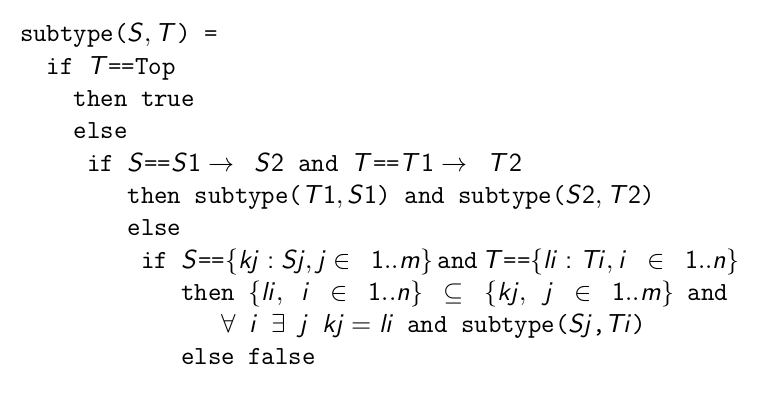
\includegraphics[scale=0.4]{imagenes/algoritmo_subtipado.png}

\subsection{Subtipado de referencias}
Queremos encontrar el tipo $Ref~\tau$ que sea subtipo de $Ref~\sigma$. 
\begin{itemize}
	\item Supongamos que $\tau <: \sigma$, si intentamos subtipar una referencia $M:Ref~\sigma$ con $Ref~\tau$, entonces cuando realicemos una asignación podremos usar un valor de tipo $\tau$ y no tendremos error. Sin embargo, cuando derreferenciemos $M$, estaremos esperando algo de tipo $\sigma$ pero como $\tau$ es más general puede tener valores que no son de ese tipo y podriamos obtener un error.
	
	\paragraph{Ejemplo:}\begin{align*}
	&\lambdaLetI{r}{\text{ref}~3}{r := 2.1}; \\
	&!r
	\end{align*}
	Como definimos $r$ como una referencia de enteros en el let, cuando derreferenciemos $r$ esperamos conseguir un entero, sin embargo la regla covariante, hace que con la asignación podamos asignar a $r$ un $Float$.
	
	\item Si  $\sigma <: \tau$ y $M: Ref~\sigma$, entonces podemos guardar en $M$ un elemento de tipo $\sigma$. Cuando querramos derreferenciar $M$, como $Ref~\sigma$ es subtipo de $Ref~\tau$, podriamos usar la derreferencia del segundo tipo. El problema vuelve a ser el mismo, el contexto va a estar esperando un valor de tipo $\tau$ y $\sigma$ es más general por lo que el valor almacenado en $M$ puede no ser de este tipo, lo que llevaría a un error.
	
	\paragraph{Ejemplo:}\begin{align}
	\lambdaLetI{r}{\text{ref}~2.1}{!r}
	\end{align}
	
	Definimos a $r$ como una referencia de $Float$. Como $r$ es subtipable a $Ref~Int$, podemos usar la derreferenciación de enteros para derreferenciarla, lo que provocaría el error en el programa.
	
\end{itemize}

Concluimos que la regla de subtipado de referencias no es ni contravariante ni covariente, es variante. La única ``sustitución" que podemos hacer es cuando $\sigma$ y $\tau$ son el mismo tipo.

$$\frac{\sigma <: \tau\hspace*{5mm} \tau <: \sigma}{Ref~\tau <: Ref~\sigma}$$

\subsubsection{Refinando el tipo \textit{Ref}}
Extendemos el lenguaje, con los siguiente tipos $Source~\sigma$ y $Sink~\sigma$ que representan las referencias de lectura y las de escritura, respectivamente. 

\paragraph{Reglas de tipado}

\begin{align*}
\frac{\judgeType{\Gamma|\Sigma}{M}{Source~\sigma}}{\judgeType{\Gamma|\Sigma}{!M}{\sigma}}(\text{T-DeRefSource})
\end{align*}

\begin{align*}
\frac{\judgeType{\Gamma|\Sigma}{M}{Sink~\sigma}\hspace*{5mm} \judgeType{\Gamma|\Sigma}{N}{\sigma}}{\judgeType{\Gamma|\Sigma}{M := N}{Unit}}(\text{T-AssignSink})
\end{align*}

\paragraph{Reglas de subtipado}
\begin{align*}
\frac{\sigma <: \tau}{Source~\sigma <: Source~\tau}(\text{S-Source})\hspace*{1cm}\frac{\tau <: \sigma}{Sink~\sigma <: Sink~\tau}(\text{S-Sink})
\end{align*}

\begin{align*}
\frac{}{Ref~\tau <: Source~\tau}(\text{S-RefSource})\hspace*{1cm}\frac{}{Ref~\tau <: Sink~\tau}(\text{S-RefSink})
\end{align*}
La regla S-Source es covariante.Si esperamos leer de una referencia de tipo $\tau$, entonces podemos esperar una referencia de un tipo más especifico que $\tau$. 

La regla S-Sink es contravariante. Cuando querramos guardar un valor de tipo $\tau$, podremos guardarlo en una referencia de este tipo o en una de un tipo más general.

Además, $Source~\tau$ y $Sink~\tau$ son menos generales que $Ref~\tau$ ya que siempre podremos remplazar referencias de lecturas o de escritura por referencias de lectura y escritura.

\newpage
\part{Paradigma orientado a objetos}
\section{Objetos y el modelo de cómputo}

En el parádigma orientado a objetos, todo programa es una simulación representada por una entidad u \textbf{objeto} que asocia los objetos físicos o conceptuales de un dominio del mundo real en objetos del dominio del programa. Estos objetos tienen las características y capacidades del mundo real que nos interesa modelar y se comunican entre si a través de intercambios de mensajes.

Los mensajes intercambiados son solicitudes para que el objeto \textbf{receptor} del mismo lleve a cabo una de sus operaciones. El \textbf{receptor} determinara si puede llevar a cabo dicha operación y, si puede hacerlo la ejecutará.

\subsection{Objetos}
Entonces un objeto es una entidad del programa que puede recibir un conjunto de mensajes (al que llamaremos \textbf{interfaz} o \textbf{protocolo}) que le permite determinar como llevar a cabo ciertas operaciones. Internamente, estará compuesto por un conjunto de \textbf{colaboradores internos} (tambien llamados \textbf{atributos} o \textbf{variables internas}) que determinan su \textbf{estado interno} y por un conjunto de \textbf{métodos} que describen (implementan) las operaciones que puede realizar y, si estas afectan a su estado interno, como lo hacen.

\paragraph{Principio de ocultamiento de la información}
El estado de un objeto es \textbf{privado} y solamente puede ser consultado o modificado por sus propios métodos, por lo que su implementación no depende de los detalles de implementación de otros objetos. Y la única forma que tenemos de interactuar con el mismo es enviándole los mensajes definidos en su interfaz.

\paragraph{Method dispatch} Es el método mediante el cuál, un proceso, estable la asociación entre el mensaje y el método a ejecutar. Es decir, cuando un objeto recibe un mensaje, el \textbf{method dispatch} se encarga de hallar la \textbf{declaración del método} que se pretende ejecutar. Este método puede ser \textbf{estático} (realizado en tiempo de compilación) o \textbf{dinámico} (realizado en tiempo de ejecución).

\paragraph{Corrientes de organización}
Por lo general,tratamos de agrupar los objetos en conjuntos compuestos por objetos que se comportan de manera similar para conseguir programas más concisos. Esto se puede hacer de dos formas: Mediante clasifiación o mediante prototipado.

\subsection{Clasificación}
Se usan \textbf{clases} que modelan \textbf{conceptos abstractos} del dominio del problema a resolver y definen el comportamiento y la forma de un conjunto de objetos (sus \textbf{instancias}). Todo \textbf{objeto} es una instancia de una clase.

\paragraph{Componentes de una clase}
Todas las clases tienen un \textbf{nombre} que usado para referenciarse a la misma. Dentro de ellas se definen las variables de instancias (colaboradores internos) de los objetos) y los métodos que saben responder esas instancias (sus nombres, sus parámetros y su cuerpo).

\subsubsection{Self/This}
Todas las clases tienen definida una pseudovariable que, durante la evaluación de un método, referencia al receptor del mensaje que activó dicha evaluación. No puede ser modificada por medio de una asignación y se liga automáticamente al receptor cuando comienza la evaluación del método.

\begin{minted}{smalltalk}
!classDefinition: #Node 
	instanceVariableNames: 'leftchild, rightchild'
	...
sum: 
	^ (self leftchild) sum + (self rightchild) ! !
	
!classDefinition: #Leaf 
	instanceVariableNames: 'value'
	...
sum: 
	^self value ! !

\end{minted}

Vemos que los métodos acceden a sus variables de instancia, enviándose a si mismos el mensaje asociado a cada una de ellas. En muchos lenguajes, para facilitar la escritura de un programa, la mención de \texttt{self} se hace implícitamente.

\subsubsection{Jerarquía de clases}
Cuando escribimos un programa en este paradigma, es común que creemos nuevas clases que extiendan a las ya existentes con nuevas variables de instancia o clase o que modifiquen el comportameiento de unos o varios métodos.

Para evitar tener que escribir toda una clase de cero, hacemos que la clase que estamos creando \textbf{herede} los atributos y los métodos de la clase pre-existente (la \textbf{super-clase}) que queremos extender. De esta forma, la nueva clase tendrá todo lo que tenía la super-clase y, además, las modificaciones que nosotros querramos agregarle.

La herencia define una relación transitiva por lo que si una clase $A$ tiene como super-tipo a otra clase $B$, entonces el super-tipo $C$ de $B$, entonces $C$ tambien es supertipo de $A$. Llamaremos \textbf{ancestros} a todos los supertipos de $A$ y \textbf{descendientes} a todos los tipos que tienen a $A$ como ancestro.

\subsubsection{Tipos de herencia}
Hay dos tipos de herencia: \textbf{simple} y \textbf{múltiple}. La herencia simple permite que una clase tenga una única clase padre y la única clase que no tiene padre es la clase \texttt{Object} que es la clase de la que heredan todas las demás. Mientras que la herencia múltiple deja que una clase tenga varios padres.

La mayoría de los lenguajes orientados a objetos utilizan la primera ya que la herencia múltiple complica el proceso de method dispath (que asocia los mensajes de un objeto con sus respectivos métodos). Para ver por qué pasa esto, supongamos que tenemos dos clases $A$ y $B$ incomparables y una clase $C$ que es subclase de $A$ y $B$. Si $A$ y $B$ definen (o heredan) dos métodos diferentes para un mismo mensaje $m$, entonces cuando enviemos dicho mensaje a $C$ deberíamos saber cual de los dos elegir.

Hay dos soluciones posibles a este problema:
\begin{itemize}
\item Podemos establecer un \textbf{orden de búsqueda} sobre las superclases de un clase estableciendo, de esta forma, un nivel de prioridad sobre algunas de ellas.
\item O obligar al programado a \textbf{redefinir} el método en $C$ si $C$ hereda dos métodos distintos para el mismo mensaje.
\end{itemize}

\subsubsection{Method Dispatch}

Como dijimos, el \textbf{method Dispatch} es el método mediante el cual asociamos un mensaje a su método correspondiente en el objeto. Por lo general, este método se realiza de manera dinámica, es decir se realizan durante tiempo de ejecución dependiendo del contexto sin embargo, hay situaciones en las que realizar este proceso de manera estática es necesario. 

Un ejemplo de esto, es cuando el lenguaje nos permite hacer uso de \texttt{super}, una pseudovariable que \textbf{referencia al objeto que recibe el mensaje} y \textbf{cambia} su proceso de activación al momento de recibir un mensaje.
Cuando usamos una expresión de la forma \texttt{super msg} en el cuerpo de un método $m$, el \textbf{method lookup} (la búsqueda del método realizada por el method dispath), comienze a realizarse desde el padre de la \textbf{clase anfitriona} de m.

Algunos lenguajes, además, nos permiten pasarle como parámetro una clase a partir de la que empezar de la siguiente forma: \texttt{super[A] msg}, siempre y cuando $A$ sea un ancestro de la clase anfitriona del método.

\subsection{Prototipado}
Lo lenguajes basados en prototipado de objetos se caracterizan por la ausencia de clases. Proveen constructores para la creación de objetos particulares y la herramientas necesarias para crear procedimientos que generen objetos.

En este tipo de paradigma, creamos instancias concretas que se interpretan como representantes canónicos de instancias (llamados \textbf{prototipos}) y, a partir de ellos, generamos otras intancias (\textbf{clones}) que pueden ser modificados sin afectar al prototipo.

Cuando hacemos esto hacemos lo que se llama una \textbf{shallow copy}, es decir copiamos cada atributo de un objeto $A$ en otro $B$. Es decir, si en $A$ tenemos una referencia a $C$, entonces en $B$ tendremos una referencia a $C$, no copiaremos $C$ a ningún otro objeto.

\subsubsection{Cálculo de objetos no tipado \texorpdfstring{($\varsigma$ cálculo)}{}}





\newpage
\section{Clasificación}
Se usan \textbf{clases} que modelan \textbf{conceptos abstractos} del dominio del problema a resolver y definen el comportamiento y la forma de un conjunto de objetos (sus \textbf{instancias}). Todo \textbf{objeto} es una instancia de una clase.

\paragraph{Componentes de una clase}
Todas las clases tienen un \textbf{nombre} que usado para referenciarse a la misma. Dentro de ellas se definen las variables de instancias (colaboradores internos) de los objetos) y los métodos que saben responder esas instancias (sus nombres, sus parámetros y su cuerpo).

\subsection{Self/This}
Todas las clases tienen definida una pseudovariable que, durante la evaluación de un método, referencia al receptor del mensaje que activó dicha evaluación. No puede ser modificada por medio de una asignación y se liga automáticamente al receptor cuando comienza la evaluación del método.

\begin{minted}{smalltalk}
!classDefinition: #Node 
	instanceVariableNames: 'leftchild, rightchild'
	...
sum: 
	^ (self leftchild) sum + (self rightchild) ! !
	
!classDefinition: #Leaf 
	instanceVariableNames: 'value'
	...
sum: 
	^self value ! !

\end{minted}

Vemos que los métodos acceden a sus variables de instancia, enviándose a si mismos el mensaje asociado a cada una de ellas. En muchos lenguajes, para facilitar la escritura de un programa, la mención de \texttt{self} se hace implícitamente.

\subsection{Jerarquía de clases}
Cuando escribimos un programa en este paradigma, es común que creemos nuevas clases que extiendan a las ya existentes con nuevas variables de instancia o clase o que modifiquen el comportameiento de unos o varios métodos.

Para evitar tener que escribir toda una clase de cero, hacemos que la clase que estamos creando \textbf{herede} los atributos y los métodos de la clase pre-existente (la \textbf{super-clase}) que queremos extender. De esta forma, la nueva clase tendrá todo lo que tenía la super-clase y, además, las modificaciones que nosotros querramos agregarle.

La herencia define una relación transitiva por lo que si una clase $A$ tiene como super-tipo a otra clase $B$, entonces el super-tipo $C$ de $B$, entonces $C$ tambien es supertipo de $A$. Llamaremos \textbf{ancestros} a todos los supertipos de $A$ y \textbf{descendientes} a todos los tipos que tienen a $A$ como ancestro.

\subsection{Tipos de herencia}
Hay dos tipos de herencia: \textbf{simple} y \textbf{múltiple}. La herencia simple permite que una clase tenga una única clase padre y la única clase que no tiene padre es la clase \texttt{Object} que es la clase de la que heredan todas las demás. Mientras que la herencia múltiple deja que una clase tenga varios padres.

La mayoría de los lenguajes orientados a objetos utilizan la primera ya que la herencia múltiple complica el proceso de method dispath (que asocia los mensajes de un objeto con sus respectivos métodos). Para ver por qué pasa esto, supongamos que tenemos dos clases $A$ y $B$ incomparables y una clase $C$ que es subclase de $A$ y $B$. Si $A$ y $B$ definen (o heredan) dos métodos diferentes para un mismo mensaje $m$, entonces cuando enviemos dicho mensaje a $C$ deberíamos saber cual de los dos elegir.

Hay dos soluciones posibles a este problema:
\begin{itemize}
\item Podemos establecer un \textbf{orden de búsqueda} sobre las superclases de un clase estableciendo, de esta forma, un nivel de prioridad sobre algunas de ellas.
\item O obligar al programado a \textbf{redefinir} el método en $C$ si $C$ hereda dos métodos distintos para el mismo mensaje.
\end{itemize}

\subsubsection{Method Dispatch}

Como dijimos, el \textbf{method Dispatch} es el método mediante el cual asociamos un mensaje a su método correspondiente en el objeto. Por lo general, este método se realiza de manera dinámica, es decir se realizan durante tiempo de ejecución dependiendo del contexto sin embargo, hay situaciones en las que realizar este proceso de manera estática es necesario. 

Un ejemplo de esto, es cuando el lenguaje nos permite hacer uso de \texttt{super}, una pseudovariable que \textbf{referencia al objeto que recibe el mensaje} y \textbf{cambia} su proceso de activación al momento de recibir un mensaje.
Cuando usamos una expresión de la forma \texttt{super msg} en el cuerpo de un método $m$, el \textbf{method lookup} (la búsqueda del método realizada por el method dispath), comienze a realizarse desde el padre de la \textbf{clase anfitriona} de m.

Algunos lenguajes, además, nos permiten pasarle como parámetro una clase a partir de la que empezar de la siguiente forma: \texttt{super[A] msg}, siempre y cuando $A$ sea un ancestro de la clase anfitriona del método.

\newpage

\section{Prototipado}
Lo lenguajes basados en prototipado de objetos se caracterizan por la ausencia de clases. Proveen constructores para la creación de objetos particulares y la herramientas necesarias para crear procedimientos que generen objetos.

En este tipo de paradigma, creamos instancias concretas que se interpretan como representantes canónicos de instancias (llamados \textbf{prototipos}) y, a partir de ellos, generamos otras intancias (\textbf{clones}) que pueden ser modificados sin afectar al prototipo.

Cuando hacemos esto hacemos lo que se llama una \textbf{shallow copy}, es decir copiamos cada atributo de un objeto $A$ en otro $B$. Es decir, si en $A$ tenemos una referencia a $C$, entonces en $B$ tendremos una referencia a $C$, no copiaremos $C$ a ningún otro objeto.

\subsection{Cálculo de objetos no tipado \texorpdfstring{($\varsigma$ cálculo)}{}}
Usaremos un lenguaje cuya única estructura computacional son los \textbf{Objetos}. Estos objetos son una colección de atributos nombrados (\textbf{registros}) que están asociados a métodos con una única variable ligada (que representa a \texttt{self}/\texttt{this}) y un cuerpo que produce un resultado.

Todos los objetos proveen dos operaciones:

\paragraph{Envío de mensajes:} Que nos permite invocar un método para que el objeto ejecute.

\paragraph{Redefinición de un método:} Que nos permite reemplazar el cuerpo de un atributo por otro.

\subsubsection{Sintaxis}
\begin{tabular}{lllll}
	$a,b$ &$::=$& &$x$ & Variables \\
 	      &     & $|$ &$[\OOAtributo{l_i}{x_i}{b_i}^{i\in1..n}]$ &  Objetos\\
 	      &     & $|$ &$a.l$ &  Selección/ Envío de mensajes \\
 	      &     & $|$ &$\OORedefinicion{a.l}{x}{b}$ &  Redefinición de un método.	       	       	      
\end{tabular}

\vspace*{5mm}
El objeto $[~]$ es el objeto vacío y no proporciona ningún método.

En este lenguajes, como todos los átributos son métodos, simulamos los colaboradores internos de un objeto con métodos que no utilizan el parámetro \texttt{self}. Por ejemplo:

$$o \equalDef [\OOAtributo{l_1}{x_1}{[~]},~
				\OOAtributo{l_2}{x_2}{x_2.l_1}]$$

$o.l_1$ retorna un objeto vacío. Y $o.l_2$ envia el mensaje $l_1$ a \texttt{self} (representado por el parámetro $x_2$). 

\paragraph{Notación} Cuando un objeto tenga un atributo de la forma $\OOAtributo{l}{x}{b}$ y $x$ no se usa en $b$ podemos escribir $l = b$ y a la reasignación $\OORedefinicion{o.l}{x}{b}$ como $o.l := b$.

\paragraph{Variables libres}
$\varsigma$ es un ligador de variables, cuando lo usamos en una expresión de la forma $\varsigma(x)b$ siempre liga la variable $x$ que se le pasa como párametro a \texttt{self}. Osea que cuando $x$ aparece en $b$ será remplazada por \texttt{self}.

De manera análoga a $FV$ del cálculo $\lambda$ definimos fv para objetos y diremos que un término $a$ es \textbf{cerrado} si fv($a$) = $\emptyset$:

\begin{center}
\begin{tabular}{ll}
	$\text{fv}(\varsigma(x)b)$ &$= \text{fv}(b)\backslash \{x\} $\\
	$\text{fv}(x)$ &$= \{x\} $\\
	$\text{fv}([\OOAtributo{l_i}{x_i}{b_i}^{i\in 1..n}])$ &$=  \bigcup^{1\in 1..n} \text{fv}(\varsigma(x)b)$\\
	$\text{fv}(a.l)$ &$= \text{fv}(a) $\\
	$\text{fv}(\OORedefinicion{a.l}{x}{b})$ &$= \text{fv}(a.l)\cup \text{fv}(\varsigma(x)b) $\\
\end{tabular}
\end{center}
\paragraph{Sustitución} La función de sustitución de variables libres para objetos está definida de la siguiente forma:

\begin{center}
\begin{tabular}{lll}
	$x\{x \leftarrow c\}$ &$= c$ & \\
	$y\{x \leftarrow c\}$ &$= y$ & si $x\neq y$\\
	$([\OOAtributo{l_i}{x_i}{b_i}^{i\in 1..n}])\{x \leftarrow c\}$ &$=  [l_i = (\varsigma(x_i)b_i)\{x \leftarrow c\}^{i\in 1..n}]$ & \\
	$(a.l)\{x \leftarrow c\}$ &$= (a\{x \leftarrow c\}).l $ & \\
	$(\OORedefinicion{a.l}{x}{b})\{x \leftarrow c\}$ &$= (a\{x \leftarrow c\}).l \leftleftharpoons (\varsigma(x)b)\{x \leftarrow c\} $ & \\
	$(\varsigma(y)b)\{x \leftarrow c\}$ &$= (\varsigma(y')(b\{y \leftarrow y'\}\{x \leftarrow c\})) $ & si $y'\notin$fv$(\varsigma(y)b)\cup$fv$(c)\cup\{x\}$ \\
\end{tabular}
\end{center}

Notemos que en el último caso, remplazamos $y$ por $y'$ por si $y = x$ asegurandonos, de esta manera, que no cambiamos el significado de la expresión.

\paragraph{$\alpha$-converión} En objetos decimos que dos métodos son equivalentes, si tienen el mismo cuerpo salvo renombre de variables, es decir: $\varsigma(x)b$ y $\varsigma(y)(b\{x\leftarrow y\})$ con $y\notin~\text{fv}(b)$ son equivalentes.

Además, dos objetos $o_1$ y $o_2$ son considerados equivalentes ($o_1 \equiv o_2$) si solo difieren en el orden se sus componentes. Si 

\begin{align*}
	o_1 \equalDef [l_1 = [~],~\OOAtributo{l_2}{x_2}{x_2.l_1}] \\
	o_2 \equalDef [\OOAtributo{l_2}{x_3}{x_3.l_1}, l_1 = [~]]
\end{align*}

son equivalentes porque ambos objetos tiene los atributos $l_1$ y $l_2$ y $\varsigma(x_2) x_2.l_1 =_\alpha \varsigma(x_3) x_3.l_1$.


\subsubsection{Semántica operacional}
Todos los objetos son considerados valores.
$$V~::=~[\OOAtributo{l_i}{x_i}{b_i}^{1\in 1..n}]$$

A diferencía del cálculo $\lambda$, usaremos el método de reducción \textbf{big-step} para evaluar expresiones, que en un solo paso nos permite saber el valor que representa.

$$\frac{}{v\longrightarrow v}[\text{Obj}]$$
\vspace*{5mm}
$$\frac{a\longrightarrow v'\hspace*{5mm} v'\equiv [\OOAtributo{l_i}{x_i}{b_i}^{i\in 1..n}]\hspace*{5mm} b_j\{x_j\leftarrow v'\}\longrightarrow v\hspace*{5mm} j\in1..n}{a.l_j\longrightarrow v}[\text{Sel}]$$

\vspace*{5mm}
$$\frac{a\longrightarrow [\OOAtributo{l_i}{x_i}{b_i}^{i\in 1..n}]\hspace*{5mm} j\in1..n}{\OORedefinicion{a.l_j}{x}{b}\longrightarrow [\OOAtributo{l_j}{x}{b},~\OOAtributo{l_i}{x_i}{b_i}^{i\in 1..n-\{j\}}]}[\text{Upd}]$$


La regla Obj nos dice que un objeto no reducen.

Sel nos indica que el resultado de enviar un mensaje es el valor que obtenemos al remplazar el párametro del método por el mismo objeto (esto es la ligación a \texttt{self}).

Upd es el comportamiento de la redifinición, que devuelve un objeto con los mismos atributos que $a$ pero remplazando el $j-$ésimo atributo por la nueva definición.


\paragraph{Ejemplo de reducción}

\begin{center}
	\begin{scprooftree}
		\def\extraVskip{5pt}
		\AxiomC{$\OOReduccion{o}{o}$}
			
			\AxiomC{$\OOReduccion{o}{o}$}
			
				\AxiomC{}
			\RightLabel{[Obj]}
			\UnaryInfC{$\OOReduccion{[~]\{x\leftarrow o\}}{[~]}$}
			\RightLabel{[Sel]}
		\BinaryInfC{$\OOReduccion{(x.a)\{x\leftarrow o\}}{[~]}$}
		
		\RightLabel{[Sel]}
		\BinaryInfC{$\OOReduccion{[a=[~],~\OOAtributo{b}{x}{x.a}].b}{[~]}$}
	\end{scprooftree}
\end{center}

\paragraph{Indefinición} Similar al cálculo lambda, podemos definir expresiones que se indefinen pero, en este caso, no es necesario que introduzcamos ninguna estructura nueva. Simplemente podemos $[\OOAtributo{a}{x}{x.a}].a$ y con esto ya alcanza.

\paragraph{Codificación de funciones (Cálculoa $\lambda$)}
Las expresiones son objetos con un atributo $val$ que nos indica su valor, las funciones, además tiene el atributo $arg$ que representa al argumento de la función. El argumento de una función permanecerá indefinido hasta que aparezca en una aplicación.
\begin{align*}
\OORep{x} &\equalDef x\\
\OORep{M~N} &\equalDef \OORep{M}.arg :=~\OORep{N}\\
\OORep{\lambdaAbsI{x}{M}} &\equalDef 
[\OOAtributo{val}{y}{\OORep{M}\{x\leftarrow y.arg\}},~\OOAtributo{arg}{y}{y.arg}]\\
\end{align*}

Cuando querramos representar un método que espera parámetros, usaremos la definición de función para escribirlo: $\varsigma(x)\OORep {\lambdaAbsI{x}{M}}$. Y podemos hacer abuso de notacion y escribir $\lambda(X)M$ y $M(N)$, en vez de $\OORep{M~N}$.

\subsubsection{Traits}
Un trait es una colección de métodos que parametrizan cierto comportamientos. Estos objetos no especifican variables de estado ni acceden a su estado.

El trait y sus métodos por si solo no son utilizables, ya que el trait no provee los estados necesarios para evaluarlos correctamente. Solo lo usaremos para definir métodos que pueden ser evaluados por varios objetos con el objetivo de no tener que repetir siempre las mismas definiciones.

Los vamos a representar como una colección de \textbf{pre-metodos} (que no usan el parámetro \text{self}). Por lo que un trait tendrá la forma:
$$\texttt{t} = [l_i = \lambdaAbsI{y_i}{b_i}^{i\in 1..n}]$$

Y, además, definimos $new$ como un constructor de objetos que crea un objeto con las mismas etiquetas que el trait y que asocia a cada una de ellas un método que invoca al método del trait con el primer parámetro ligado a \texttt{self}:

$$new \equalDef \lambdaAbsI{z}{[\OOAtributo{l_i}{s}{z.l_i(s)^{i\in 1..n}}]}$$

Veamos un ejemplo, definimos el trait \texttt{CompT}:

\begin{align*}
	\texttt{CompT}\equalDef [~& \\ &\OOAtributo{eq}{t}{\lambda(x)\lambda(y)\lambdaIf{(x.comp(y)) == 0}{\texttt{true}}{\texttt{false}}},~\\
	&\OOAtributo{leq}{t}{\lambda(x)\lambda(y)\lambdaIf{(x.comp(y)) < 0}{\texttt{true}}{\texttt{false}}} \\
	]~&
\end{align*}

Entonces $new~\texttt{CompT}$ reduce a:
\begin{align*}
new~\texttt{CompT}\longrightarrow [~& \\ &\OOAtributo{eq}{x}{\lambda(y)\lambdaIf{(x.comp(y)) == 0}{\texttt{true}}{\texttt{false}}},~\\
&\OOAtributo{leq}{x}{\lambda(y)\lambdaIf{(x.comp(y)) < 0}{\texttt{true}}{\texttt{false}}} \\
]~&
\end{align*}

\paragraph{Clase} Cuando un trait provee un método $new$, diremos que es un \textbf{trait completo} o \textbf{clase}.

\begin{align*}
\texttt{C}\equalDef [~& \\ &\OOAtributo{new}{z}{[\OOAtributo{l_i}{s}{z.l_i(s)^{i\in 1..n}}]}~\\
&\OOAtributo{leq}{t}{\lambda(x)\lambda(y)\lambdaIf{(x.comp(y)) < 0}{\texttt{true}}{\texttt{false}}} \\
]~&
\end{align*}

\paragraph{Herencia} Cuando queremos que una clase ``herede'', lo que hacemos es crear un nuevo trait que contenga todas las etiquetas del trait original y asocie cada una de esas etiquetas al método correspondiente del trait original y le agregamos los atributos que deseamos para extenderlo. Además, modificamos el constructor $new$ para que tome en cuenta los nuevos atributos.

Por ejemplo, la clase contador:

\vspace*{5mm}
\begin{tabular}{ll}
$\texttt{Contador}\equalDef [$ &
$new = \varsigma(z)[\OOAtributo{inc}{s}{z.inc(s)},~v = 0,~ \OOAtributo{get}{s}{z.get(s)} ],$ \\
 & $inc = \lambda(s) s.v := s.v + 1,$ \\
 & $get = \lambda(s) s.v$ \\
  & $]$ \\
\end{tabular}

Y su sublcase \texttt{ContadorR}:

\vspace*{5mm}
\begin{tabular}{ll}
$\texttt{ContadorR}\equalDef [$ &
$new = \varsigma(z)[$
\\ & $\quad\OOAtributo{inc}{s}{z.inc(s)},$ \\ 
 & $\quad v = 0,$ \\
 & $\quad \OOAtributo{get}{s}{z.get(s)},$ \\
 & $\quad \OOAtributo{reset}{\lambda(s)}{z.reset(s)} $ \\
 & $ ],$ \\
& $inc = \texttt{Contador}.inc$ \\
& $get = \texttt{Contador}.get$ \\
& $reset = \lambda(s) s.v := 0,$ \\
& $]$ \\
\end{tabular}


\paragraph{Otras consideraciones del lenguaje}
El lenguaje que definimos se parece mucho al funcional. En la versión imperativa, donde se mantiene un store con referencias a objetos, se ofrece la función \texttt{Clone}$(a)$ que crea un nuevo objeto con las mismas etiquetas de $a$ y cada componente comparte los métodos con las componentes de $a$.

Además, el lenguaje no nos deja agregar o eliminar dinámicamente métodos en un objeto. No nos deja extraer los métodos de los objetos.

Hay otras versiones de este cálculo que incluyen sistemas de tipado.

\newpage
\part{Paradigma Lógico}
En este paradigma, las programas son un conjunto \textbf{hechos} y \textbf{reglas de inferencia} que sirven para inferir si un \textbf{objetivo} o \textbf{goal} es consecuencia de ellos. Es decir que, cuando escribimos un programa, \textbf{declaramos} expresiones que sabemos que son verdad (hechos y reglas) que nos permitirán probar, a través del uso de la lógica, que una expresión (objetivo) es verdad.

En prolog, esta demostración, se hace a través de un motor de inferencia que se basa en el \textbf{método de resolución} para realizar la demostración. Vamos a ver métodos no deterministicos de resolución para expresiones de la lógica proposicional y de primer orden. Luego, agregaremos a estos métodos reglas que nos permitirán convertirlos en algoritmos determinísticos y las formas y condiciones que debe cumplir un programa para que sea compatible con estas reglas.

\section{Lógica Proposicional}
\subsection*{Sintaxis}
Dado un conjunto $\mathcal{V}$ de \textbf{variables proposionales} $P,P_0,P_1,\dots$, el conjunto de \textbf{formulas proposicionales (o proposiciones)} se define como:

\begin{align*}
		A,B ~ :&= ~ P &&\text{una variable proposicional} \\
		& |~ \lnot A &&\text{negación}\\
		& |~ A \land B &&\text{conjunción}\\
		& |~ A \lor B &&\text{disjunción}\\
		& |~ A \supset B &&\text{implicación}\\
		& |~ A \iff B &&\text{si y solo si} \\
\end{align*}


\subsection{Semántica} 

Una \textbf{evaluación} es una función $v:\mathcal{V}\to{\textbf{T},\textbf{F}}$ que asigna valores de verdad a las variables proposicionales. Decimos que $v$ \textbf{satisface} una proposicón $A$ si $V\models A$ donde:

\begin{align*}
v \models P~&sii~v(P) = T\\
v \models \lnot A~&sii~ v \not{\models} A \text{ ($v$ no satisface $A$)}\\
v \models A \lor B~&sii~v \models A \text{ o } v\models B\\
v \models A \land B~&sii~v \models A \text{ y } v\models B\\
v \models A \supset B~&sii~v\not\models A \text{ o } v\models B\\
v \models A \iff B~&sii~(v\models A \text{ sii } v\models B)\\
\end{align*}

Una proposición es \textbf{satisfactible} si existe una valuación $v$ tal que $v\models A$. Cuando no existe $v$ qua satisfaga $A$, decimos que $A$ es \textbf{insatisfactible}.

Podemos extender estas definiciones a conjuntos de proposiciones. Si $S$ es un conjunto de proposiciones, entonces es \textbf{satisfactible} si existe una valuación $v$ tal que para todo $A\in S$, se tiene que $v\models A$. Y si no existe este $v$, entones $S$ es \textbf{insatisfactible}.

Dada una proposición $A$, si vale que $v\models A$ para toda valuación $v$, entonces decimos que $A$ es una \textbf{tautología}.

\paragraph{Literales} Un literal es una variable proposicional $P$ o su negación $\lnot P$.

\subsubsection{Forma Normal Conjutiva (FNC)}\label{Logica::Proposicional::FNC}
Diremos que una proposición $A$ está en FNC si es una conjunción de disjunciones de literales. Es decir si tiene la siguiente forma:

$$C_1 \land\dots\land C_n$$

donde cada \textbf{claúsula} $C_i$ es una disyunción de literales:

$$B_{i1}\lor\dots\lor B_{in_i}$$

\paragraph{Teorema:} Para toda proposición $A$ puede hallarse una proposición $A'$ en FNC que es lógicamente equivalente a $A$.

\paragraph{Nota:} $A$ es lógicamente equivalente a $B$ si y solo si la proposición $A\iff B$ es una tautología. 

\subsubsection*{Notación conjuntista}
Dada la siguiente expresión en forma normal conjuntiva:

$$(A\lor B)\land(A\lor \lnot A) \land (\lnot B \lor \lnot B) \land (B\lor A)\land (C\lor D)$$
 
Trataremos de escribirla de manera más simple. Lo primero que notamos es que $(A \lor \lnot A)$ es una tautología, ya que siempre vale una de las dos propocisiones. Entonces podemos eliminar esta clausula sin modificar su valor de verdad.

$$(A\lor B)\land (\lnot B \lor \lnot B) \land (B\lor A)$$

Además, $(\lnot B \lor \lnot B) \iff \lnot B$ ($\lor$ es idempotente):

$$(A\lor B)\land \lnot B \land (B\lor A)$$

Como $\lor$ también es conmutativo, sabemos que $(A \lor B) \iff (B \lor A)$ por lo que podemos eliminar una de las dos:

$$(A\lor B)\land \lnot B$$

Logramos escribir la proposición original con una expresión equivalente con todas las clausulas distintas. Donde las clausula son $C_1 = (A\lor B)$ y $C_2 = \lnot B$.

Cuando sucede esto, podemos representar la proposición como un conjunto de clausulas \\ $\{C_1,\dots,C_n\}$ donde cada clausula $C_i$ es un conjunto de literales. Es decir que la expresión del ejemplo puede ser escrita de la siguiente manera:

$$\{\{A,B\},\{\lnot B\}\}$$

\subsection{Validez por refutación}

\textbf{Teorema:} Una proposición $A$ es una tautología sii $\lnot A$ es insastisfactible.

\vspace*{5mm}
Entonces, dada una proposición $A$, si probramos que $\lnot A$ es insatisfactible podemos probar que $A$ es una tautología. A pesar de que hay varias técnicas para hacer esto, vamos a concentrarnos en el método de \textbf{resolución} que fue introducipo por Alan Robinson en 1965.

Este método es simple de implementar y hace uso de una única regla de inferencia (\textbf{la regla de resolución}) para demostrar que una fórmula en forma normal conjuntiva es insatisfactible.

\subsubsection{Principios fundamentales}
El método, usa la regla de inferencia para expandir un conjunto $S$ hasta que el mismo contenga dos clausulas que se niegen entre si. Para esto, hace uso de la siguiente tautología: 

$$(A\lor P)\land (B\lor \lnot P) \iff (A\lor P)\land (B\lor \lnot P) \land (A \lor B)$$

\begin{centrado}
\paragraph{Demostración} Queremos ver que $(A\lor P)\land (B\lor \lnot P)$ y $(A\lor P)\land (B\lor \lnot P) \land (A \lor B)$ son equivalentes:

Si $(A\lor P)\land (B\lor \lnot P)$ es satisfactible, entonces valen las dos clausulas de la proposición. Por la primer clausula vale que $A$ es satisfactible o $P$ lo és. Si $P$ es satisfactible, entonces $B$ es satisfactible, pues $\lnot P$ no lo es, entonces vale $(A\lor B)$.

Si $P$ no es satisfactible, entonces $A$ debe serlo para que $(A\lor P)$ lo sea y, además $\lnot P$ es satisfactible por lo que la segunda clausula tambien lo és y como $A$ es satisfactible vale $(A\lor B)$.

Por otro lado, si $A$ y $B$ no son satisfactibles, entonces $(A\lor P)\land (B\lor \lnot P)$ no es satisfactible pues, para que lo sea, tendrían que valer $P$ y $\lnot P$ al mismo tiempo.

Entonces, ambas expresiones son equivalentes.

\end{centrado}

Este resultado nos permite asegurar que los conjuntos de claúsulas 
$$\{C_1,\dots,C_n,\{A,P\}, \{B,\lnot P\}\}\hspace*{5mm}y\hspace*{5mm}\{C_1,\dots,C   _n,\{A,P\}, \{B,\lnot P\}, \{A,B\}\}$$
son equivalentes. Y si uno de ellos es insatisfactible, entonces el otro lo és.

Cuando esto suceda, diremos que la cláusula $\{A,B\}$ es la \textbf{resolvente} de las claúsulas $\{A,P\}$ y $\{B,\lnot P\}$. Además generalizamos la definicion para clausulas con más de dos literales:

\paragraph{Notación:} Dado un literal $L$,  su opuesto $\overline{L}$ se define como
\begin{itemize}
\item  $\lnot P$ si $L=P$ 
\item $P$ si $L=\lnot P$.
\end{itemize}


\vspace*{5mm}
Dadas dos cláusulas $C_1$, $C_2$, una claúsula $C$ se dice \textbf{resolvente de $C_1$ y $C_2$} si y solo si, para algún literal $L$, $L\in C_1$ y $\overline{L}\in C_2$ y $C = (C_1-\{L_1\})\cup(C_2-\{\overline{L}\})$. Notaremos la regla de resolución como
$$\frac{C_1 = \{A_1,\dots,A_m,L\}\hspace*{5mm} C_2 = \{B_1,\dots,B_m, \overline{L}\}}{C = \{A_1,\dots,A_m, B_1,\dots,B_n\}}$$


El método de resolución ira agregando resolventes (que todavía no pertenezcan) al conjunto hasta conseguir un conjunto que contenga dos cláusulas de la forma $\{P\}$ y $\{\lnot P\}$ cuya resolvente es la cláusula vacía notada como $\Box$. Cuando esto suceda, diremos que conseguimos una \textbf{refutación}.

Entonces, en resumen, el método de resolución trata de construir una secuencia de conjuntos claúsales que termina en una refutación y, si lo logra, como todos los conjuntos de la secuencia son equivalentes el conjunto original no es satisfactible.

El método siempre termina, ya que las resolventes agregados se forman con los literales distintos que aparecen en el conjunto de partida y hay una cantidad finitas de literales en dicho conjunto.

En el peor de los casos, la regla de resolución podrá generar una nueva cláusula por cada combinación diferente de literales distintos de $S$.

\paragraph{Teorema} Dado un conjunto finito $S$ de cláusulas, $S$ es insatisfactible si y solo si tiene una refutación. 

\subsubsection*{Ejemplo de resolución}

Vamos a probar que $\{ \{P,Q\},\{P,\lnot Q\},\{\lnot P, Q\},\{\lnot P, \lnot Q\}\}$ es insatisfactible. Armamos la primer resolvente con $\{P,Q\}$,$\{P,\lnot Q\}$ que nos queda $C = \{P\}$, entonces el nuevo conjunto es:
$$\{ \{P,Q\},\{P,\lnot Q\},\{\lnot P, Q\},\{\lnot P, \lnot Q\}, \{P\} \}$$
Armamos la segunda resolvente con $\{\lnot P, Q\}$ y $\{\lnot P, \lnot Q\}$ entonces $C_1 = \{\lnot P\}$:
$$\{ \{P,Q\},\{P,\lnot Q\},\{\lnot P, Q\},\{\lnot P, \lnot Q\}, \{P\}, \{\lnot P\} \}$$
Y por útlimo usamos $\{P\}$ $\{\lnot P\}$ y agregamos la resolvente $\Box$ al conjunto, obteniendo de esta manera la refutación que buscabamos.

$$\{ \{P,Q\},\{P,\lnot Q\},\{\lnot P, Q\},\{\lnot P, \lnot Q\}, \{P\}, \{\lnot P\}, \red{\Box} \}$$


\newpage
\section{Lógica de primer orden}
Definimos un método para probar que una proposición es una tautología. Sin embargo, todavía no tiene todo el poder que podría tener. Nos gustaría, dada una proposición con literales, saber que valor deberían tomar esos literales para que la proposición sea una tautología.

Para esto debemos dotar de semántica a los literales y proveer un mecanismo que nos permita inferir los valores que deben componer a cada uno de ellos.

\subsection{Repaso}
Un \textbf{lenguaje de primer orden} (LPO) $\mathcal{L}$ consiste en:
\begin{enumerate}
\item Un conjunto numerable de \textbf{constantes} $c_0,c_1,\dots$
\item Un conjunto numerable de \textbf{símbolos de función} con aridad $n > 0$ $f_0, f_1,\dots$
\item Un conjunto numerable de \textbf{símbolos de predicado} con aridad $n\geq 0$, $P_0,P_1,\dots$.
\end{enumerate}

\subsubsection{Términos de primer orden}
Sea $\mathcal{V} = \{x_0,x_1,\dots\}$ un conjunto numerable de variables y $\mathcal{L}$ un lenguaje de primer orden. El conjunto de \textbf{$\mathcal{L}$-términos} se define inductivamente como:
\begin{itemize}
\item Toda constante de $\mathcal{L}$ y toda variable es un $\mathcal{L}$-término.
\item Si $t_1,\dots,t_n\in \mathcal{L}$-términos y $f$ es un símbolo de función de aridad $n$, entonces $$f(t_1,\dots,t_n)\in \mathcal{L}\text{-términos}$$
\end{itemize}

\subsubsection{Fórmulas átomicas}
Sea $\mathcal{V}$ un conjunto numerable de variables y $\mathcal{L}$ un lenguaje de primer orden. El conjunto de \textbf{$\mathcal{L}$-fórmulas átomicas} se define inductivamente como:
\begin{enumerate}
\item Todo símbolo de predicado de aridad $O$ es una $\mathcal{L}$-fórmula átomica.
\item Si $t_1,\dots,t_n\in\mathcal{L}$-términos y $P$ es un símbolo de predicado de aridad $n$, entonces $P(t_1,\dots,t_n)$ es una $\mathcal{L}$-fórmula átomica.
\end{enumerate}
\subsubsection{Fórmulas de primer orden}
Sea $\mathcal{V}$ un conjunto numerable de variables y $\mathcal{L}$ un lenguaje de primer orden. El conjunto de \textbf{$\mathcal{L}$-fórmulas} se define inductivamente como:
\begin{enumerate}
\item Toda $\mathcal{L}$-fórmula átomica es $\mathcal{L}$-fórmula.
\item Si $A,B\in \mathcal{L}$-fórmula, entonces $\lnot A$, $(A\land B)$, $(A\lor B)$, $(A\supset B)$ y $A\iff B$ son $\mathcal{L}$-fórmulas.
\item Para toda variable $x_i$ y cualquier $\mathcal{L}$-fórmula $A$, $\forall x_i.A$ t $\exists x_i.A$ son $\mathcal{L}$-fórmulas.

\end{enumerate}
\subsubsection*{Variables libres y ligadas}

Las variables pueden ocurrir \textbf{libres} o \textbf{ligadas}. En este lenguaje, los cuantificadores ligan variable y usaremos $FV(A)$ y $BV(A)$ parar referirnos a las variables libres y ligadas, respectivamente, de $A$.

Cuando $FV(A) = \emptyset$ diremos que $A$ es una \textbf{sentencia}.

Una fórmula $A$ está \textbf{rectificada} si $FV(A)$ y $BV(A)$ son disjuntos, es decir si todos los cuantificadores que aparecen en $A$ ligan variables distintas. Además, toda fórmula se puede \textbf{rectificar} a una fórmula equivalente renombrando sus variables.

\subsubsection{Estructuras de primer orden}
Dado un lenguaje $\mathcal{L}$, una \textbf{estructura para $\mathcal{L}$}, \textbf{M}, es un par \textbf{M} $=(M, I)$ donde 
\begin{itemize}
\item $M$ (\textbf{dominio}) es un conjunto no vacío
\item $I$ (\textbf{función de interpretación}) asigna funciones y predicados sobre $M$ a símbolos del lenguaje $\mathcal{L}$ de la siguiente manera:
\begin{enumerate}
\item Para toda constante $c$, $I(c)\in M$.
\item Para todo $f$ de aridad $n > O$, $I(f):M^n\to M$
\item Para todo predicado $P$ de aridad $n \geq 0$, $I(P) : M^n \to\{\textbf{T}, \textbf{F}\}$

Sea $M$ una estructura para $\mathcal{L}$. Una \textbf{asignación} es una función $s:\mathcal{V}\to M$ y, si $a\in M$, escribimos $s[x \leftarrow a]$ para denotar la asignación que se comporta igual que $s$ salvo en el elemento $x$, en cuyo caso retorna $a$.
\end{enumerate}
\end{itemize}

\subsubsection{Satisfactibilidad}
La relación $s \models_M A$ establece que la asignación $s$ satisface la fórmula $A$ en la estructura $M$. Y se define usando inducción estructural en $A$:

\begin{align*}
&s \models_\textbf{M} P(t_1,\dots,t_n)&&~sii~P(s(t_1),\dots,s(t_n))&&&\\
&s \models_\textbf{M} \lnot A &&~sii ~s \not{\models}_\textbf{M} A &&&\\
&s \models_\textbf{M} (A \lor B)&&~sii~s \models_\textbf{M} A \text{ o } s\models_\textbf{M} B&&&\\
&s \models_\textbf{M} (A \land B)&&~sii~s \models_\textbf{M} A \text{ y } s\models_\textbf{M} B&&&\\
&s \models_\textbf{M} (A \supset B)&&~sii~s\not\models_\textbf{M} A \text{ o } s\models_\textbf{M} B&&&\\
&s \models_\textbf{M} (A \iff B)&&~sii~(s\models_\textbf{M} A \text{ sii } s\models_\textbf{M} B)&&&\\
&s \models_\textbf{M} (A \supset B)&&~sii~s\not\models_\textbf{M} A \text{ o } s\models_\textbf{M} B&&&\\
&s \models_\textbf{M} \forall x_i.A &&~sii~s[x_i\leftarrow a]\models_\textbf{M} A \text{ para todo } a\in \textbf{M}&&&\\
&s \models_\textbf{M} \exists x_i.A &&~sii~s[x_i\leftarrow a]\models_\textbf{M} A \text{ para algún } a\in \textbf{M}&&&\\
\end{align*}

\newpage
\subsubsection{Validez}\label{logica::primerOrden::validez}
\begin{itemize}
\item Una fórmula $A$ es \textbf{satisfactible en M} si y solo si existe una asiganción $s$ tal que $s\models_\textbf{M} A$

\item Una fórmula $A$ es \textbf{satisfactible} si y solo si existe un \textbf{M} tal que A es satisfactible en \textbf{M}. En caso contrario se dice que $A$ es insatisfactible.

\item Una fórmula $A$ es \textbf{válida en M} si y solo si $s \models_\textbf{M} A$, para toda asigación $s$.

\item $A$ es valida si y solo si $\lnot A$ es insatisfactible.
\end{itemize}

\subsection{El método de resolución}

El \textbf{teorem de Church} asegura que \textbf{no} existe un algoritmo que pueda determinar si una fórmula de primer orden es válida. Por lo que el método de resolución será parcialmente computable, es decir que si la sentencia que deseamos resolver es insatisfactible entonces hallaremos una refutación a la misma, en caso contrario puede ser que no se detenga.

Para resolver una fórmula, el método tomará su forma clausal e irá agregando resolventes hasta que el conjunto contenga a la cláusula vacía.

\subsubsection{Forma de la fórmula}
Dada una fórmula $A$, el primer pasoe es escribirla en forma clausal siguiendo estos pasos:
\begin{enumerate}
\item Eliminar las implicaciones, es decir, si aparece una clausula de la forma $(A\supset B)$, reescribirla como $(\lnot A \lor B)$.

\item Pasar a \textbf{forma normal negada}.
\item Pasar a \textbf{forma normal prenexa}.
\item Pasar a \textbf{forma normal de Skolem}.
\item Pasar a \textbf{forma normal conjuntiva}.
\item \textbf{Distribuir} cuantificadores universales.
\end{enumerate}

\subsubsection*{Forma normal negada}
El conjunto de fórmulas en \textbf{forma normal negada} (NNF) se define inductivamente como:

\begin{enumerate}
\item Para cada fórmula atómica $A$, $A$ y $\lnot A$ están en NNF.
\item Si $A,B\in$ NNF, etnoces $(A\lor B),(A\land B) \in$ NNF.

\item Si $A\in$ NNF, entonces $(\forall x.A),(\exists x. A)\in$ NNF.
\end{enumerate}

En otras palabras, son todas las fórmulas en las que si aparece una negación, entonces esta está aplicada a una formula atómica del lenguaje.

Los remplazos que se hacen para pasar una formula a FNN son:

\begin{multicols}{2}
$$\lnot(A\land B) \iff \lnot A \land \lnot B$$
$$\lnot(A\lor B) \iff \lnot A \lor \lnot B$$
\vfill\null
\columnbreak
$$\lnot\lnot A \iff A$$
$$\lnot\forall x.A \iff \exists x.\lnot A$$
$$\lnot\exists x.A \iff \forall x.\lnot A$$
\end{multicols}

\subsubsection*{Forma normal prenexa}
Son las fórmulas de la forma $Q_1x_1\dots Q_nx_n.B$, $n\geq 0$, donde $B$ no tiene cuantificadores, $x_1,\dots,x_n$ son variables y $Q_i \in \{\forall,\exists\}$.

Sea $A$ una fórmula en forma normal negativa, entonces valen las siguientes equivalencias:

\begin{multicols}{2}
$$(\forall x.A)\land B \iff \forall x.(A\land B)$$
$$(A\land\forall x.B) \iff \forall x.(A\land B)$$
$$(\exists x.A)\land B \iff \exists x.(A\land B)$$
$$(A\land\exists x.B) \iff \exists x.(A\land B)$$

$$(\forall x.A)\lor B \iff \forall x.(A\lor B)$$
$$(A\lor\forall x.B) \iff \forall x.(A\lor B)$$
$$(\exists x.A)\lor B \iff \exists x.(A\lor B)$$
$$(A\lor\exists x.B) \iff \exists x.(A\lor B)$$
\end{multicols}

Cuando una fórmula tenga dos o más cuantificadores que liguen variables con el mismo nombre, entonces debemos renombrar cada una de esas variables con nombres distintos para poder realizar la transformación.

\subsubsection{Forma normal de Skolem}
Dada una fórmula en forma normal prenexa, debemos pasarla a forma normal de Skolem usando un proceso llamado \textbf{solemización}. El objetivo de esta transformación es eliminar los cuantificadores existenciales de un fórmula sin alterar su sastifactibilidad.

La idea es que al eliminar el existencial remplazemos cada aparición de la variable que ligaba por un ``testigo'' que es una constante nueva del lenguaje de primer orden que depende de las demás variables libres de la fórmula. Por ejemplo, si tenemos la fórmula $\exists x.P(x)$, su forma skolemizada será $P(c)$ con $c$ una nueva constante del lenguaje que llamaremos \textbf{parámetro}. 

En fórmulas más grandes,  cada ocurrencia de una subfórmula $\exists x.B$ en $A$ se remplaza por $B\{ x \leftarrow f(x_1,\dots,x_n)\}$ donde:
\begin{itemize}
\item $\{\bullet \leftarrow \bullet\}$ es la operación usual de sustitución.
\item $f$ es un símbolo de función nuevo y las $x_1,\dots, x_n$, son las variables libres en $B$ de las que depende $x$.
\end{itemize} 

Ahora, si bien el resultado de skolemizar una fórmula preserva la sastifactibilidad, no preserva validez. Por ejemplo, la fórmula $\exists x.(P(a) \supset P(x))$ es válida, sin embargo, su skolemización \\ $P(a)\supset P(b)$ no lo es. (Ver la definición de validez en \ref{logica::primerOrden::validez}).

\subsubsection*{Definición formal}
Sea $A$ una sentencia rectificada en forma normal negada, la \textbf{forma normal de Skolem de A} (\textbf{SK(A)}) se define recursivamente como sigue:

Sea $A'$ cualquier subfórmula de $A$, 
\begin{itemize}
\item Si $A'$ es una fórmula atómica o su negación, \textbf{SK}$(A') = A'$.
\item Si $A'$ es de la forma $(B\star C)$ con $\star \in \{\land,\lor\}$, entonces $\textbf{SK}(A') = (\textbf{SK}(B)\star \textbf{SK}(C))$.
\item Si $A'$ es de la forma $\forall x.B$, entonces $\textbf{SK}(A') = \forall x.\textbf{SK}(B)$.
\item Si $A'$ es de la forma $\exists x.B$ y $\{x,y_1,\dots,y_m\}$ son las variables libres de $B$, entonces:
\begin{enumerate}
\item Si $m>0$, crear un \textbf{símbolo de función de Skolem}, $f_x$ de aridad $m$ y definir:

$$\textbf{SK}(A') = \textbf{SK}(B\{ x \leftarrow f(y_1,\dots,y_m)\})$$

\item Si $m=0$, crear una nueva \textbf{constante de Skolem} $c_x$ y

$$\textbf{SK}(A') = \textbf{SK}(B\{ x \leftarrow c_x\})$$

\end{enumerate}
\end{itemize}

\subsubsection*{Forma clausal}
Una vez que tenemos una formula en forma normal prenexa skolemizada, es decir tiene la siguiente forma:
 $$\forall x_1\dots\forall x_n.B$$

Pasamos $B$ a \textbf{forma normal conjuntiva} \ref{Logica::Proposicional::FNC} como si fuese una fórmula proposicional y distribuimos los cuantificadores sobre cada conjunción, obteniendo así una conjunción de \textbf{cláusulas}

$$\forall x_1\dots\forall x_n.C_1\land\dots\land\forall x_1\dots\forall x_n.C_m$$

donde cada $C_i$ es una disyunción de literales.  Luego, podemos escribirla de la siguiente forma:

$$ \{C_1,\dots,C_m\}$$

\subsubsection{Regla de resolución}
Las variables del lenguaje nos permiten escribir expresiones que son un ``template'' que nos asegura que podemos encontrar un conjunto de constantes tal que si remplazamos las apariciones de esas variables por esas constantes y eliminamos los cuantificadores, obtenemos una verdad. Por ejemplo, si tenemos $\forall x.P(x)$, entonces vale $P(a),P(b),\dots$ (vale para cualquier constante del lenguaje). Y si tenemos $\exists x.(x < 1)$, entonces podemos encontrar constantes para lo que vale esa fórmula, en este caso $x=0$ lo cumple.

La regla de resolución debe tener en cuenta que, a pesar de que una clausula no sea negación de otra, puede haber claúsulas que sean ``instancias'' de otras y que contradigan a otras.

Por ejemplo, si tenemos $\{{P(x)\}, \{\lnot P(a)\}}$ podemos deducir que el conjunto es insatisfactible porque por la segunda cláusula vale $\lnot P(a)$ pero, por la primera vale que $\forall x.P(x) \Rightarrow P(a)$.

Entonces, debemos \textbf{unificar} estas dos expresiones para poder llegar a un error. Definimos la regla de la siguiente forma:

$$\frac{\{\blue{B_1,\dots,B_k},A_1,\dots,A_n\}\hspace*{5mm}\{\blue{\lnot D_1,\dots,\lnot D_k},A_1,\dots,A_n\}}{\red{\sigma(\{A_1,\dots A_m, C_1,\dots,C_n\})}}$$

donde $\sigma$ es el \textbf{unificador más general} (MGU) de $\{B_1,\dots,B_k,\lnot D_1,\dots,\lnot D_k\}$ y $\sigma(\{A_1,\dots A_m, C_1,\dots,C_n\})$ es el \textbf{resolvente}.

Cuando usamos $\sigma$, debemos tener en cuenta que todas las cláusulas usan variables distintas, por lo que si hay dos cláusulas que usan variables con el mismo nombre es conveniente renombrarlas para evitar confusiones.

\subsubsection{Método de resolución}

Entonces ya tenemos la regla de resolución para fórmulas de la lógica de primer orden. El método de resolución es análogo al de la lógica proposicional. En cada paso buscaremos una resolvente que podamos agregar al conjunto y haremos esto hasta que la resolvente que agregamos sea $\Box$ (la cláusula vacía).

A diferencia del método de lógica de primer orden, en cada paso no solo agregaremos una resolvente al conjunto sino que además definimos una función unificadora que nos permitirá deducir los valores que pueden tomar las variables libres de una expresión para que sea valida. Esta deducción la haremos de manera similar a como lo hacemos cuando ejecutamos el algoritmo de inferencia para tipos del cálculo $\lambda$ (una vez terminada nuestra demostración compondremos todas las sustituciones realizadas).

\paragraph{Ejemplo:} Queremos probar que $\{C_1, C_2, C_3\}$ es insatisfactible con
\begin{itemize}
\item $C_1 = \{\lnot P(z_1,a), \lnot P(z_1,x), \lnot P(x,z_1)\}$
\item $C_2 = \{P(z_2,f(z_2)), P(z_2,a)\}$
\item $C_3 = \{P(f(z_3),z_3), P(z_3,a)\}$
\end{itemize}

\begin{centrado}
\begin{enumerate}
\item De $C_1$ y $C_2$ con $\{z_1\leftarrow a, x\leftarrow a, z_2\leftarrow a,\}$ tenemos $C_4 = \{ P(a,f(a))\}$
\item De $C_1$ y $C_2$ con $\{z_1\leftarrow a, x\leftarrow a, z_3\leftarrow a,\}$ tenemos $C_5 = \{ P(f(a),a)\}$
\item De $C_1$ y $C_5$ con $\{z_1 \leftarrow f(a), x\leftarrow a\}$: $C_6 = \{ \lnot P(a,f(a))\}$
\item De $C_4$ y $C_6$: $\Box$.
\end{enumerate}
\end{centrado}

\subsubsection{Regla de resolución binaria}

$$\frac{\{\blue{B_1},A_1,\dots,A_n\}\hspace*{5mm}\{\blue{\lnot D_1},A_1,\dots,A_n\}}{\red{\sigma(\{A_1,\dots A_m, C_1,\dots,C_n\})}}$$

\hspace*{5mm}
Si intentamos refutar $\{\{P(x), P(y)\}, \{\lnot P(v), \lnot P(w)\}\}$ solo con esta regla nos encontraremos con que no podremos encontrar una secuencia de resolventes que termine en la cláusula $\Box$.

\subsubsection*{Regla de factoriazción}
La regla de factorización resuelve este problema permitiendonos extraer de una cláusula un literal represente a cada uno de los literales que la componen. Es decir, un literal que pueda ser unificado con cada uno de los literales de la cláusula.

$$\frac{\{\blue{B_1,\dots,B_k},A_1,\dots,A_n\}}{\red{\sigma(\{B_1,A_1,\dots A_m\})}}$$

\hspace*{5mm}

Entonces con esta regla podemos usar $\{P(z)\}$ como resolvente para la cláusula $\{P(x), P(y)\}$ y la demostración del ejemplo anterior quedaría de la siguiente forma:

\begin{enumerate}
\item $\{\{P(x), P(y)\}, \{\lnot P(v), \lnot P(w)\}\}$
\item $\{\{P(x), P(y)\}, \{\lnot P(v), \lnot P(w)\}, \blue{\{P(z)\}}\}$ (por la regla de factorización sobre la primer cláusula)
\item $\{\{P(x), P(y)\}, \{\lnot P(v), \lnot P(w)\}, \{P(z)\}, \blue{\{\lnot P(u)\}}\}$ (por la regla de factorización sobre la segunda cláusula)
\item $\{\{P(x), P(y)\}, \{\lnot P(v), \lnot P(w)\}, \{P(z)\}, \{\lnot P(u)\}, \Box\}$
\end{enumerate}

\newpage

\section{Resolución SLD}
Si bien los métodos que propusimos hasta ahora son completos, hallar refutaciones es un proceso muy car en el caso general, el espacio de búsqueda que producen puede ser enorme y tienen un alto grado de no-determinismo. Debemos agregar ciertas restricciones que nos permitan reducir este espacio sin que esto afecte a la completitud del método.

\subsection{Resolución lineal}
Una secuencia de pasos de resolución a partir de $S$ es \textbf{lineal} si es de la forma:

\begin{center}
	\begin{forest} resolucion,
[$C_p~{=}~\Box$ 
	[$C_{p-1}$,edge label={node[midway,right] {$\blue{\sigma_p}$}}
    	[$\dots$,edge label={node[midway,right] {$\blue{\sigma_{p-1}}$}}
        	[$C_3$,
            	[$C_2$,edge label={node[midway,right] {$\blue{\sigma_3}$}}
                	[$C_1$, edge label={node[midway,right] {$\blue{\sigma_2}$}}
           	        	[$C_0$, edge label={node[midway,right] {$\blue{\sigma_1}$}}]
                      	[$B_1$]
                	]
                	[$B_2$]        	
            	]
                [$B_3$]
        	]
    	]
    	[$B_{p-1}$]	
	]
    [$B_p$]
]
	\end{forest}
\end{center}

donde $C_0$ y cada $B_i$ es un elemento de $S$ o algún $C_j$ con $j < i$.

Este tipo de resolución reduce el espacio de búsqueda considerablemente, sin embargo sigue siendo altamanente no-deterministico ya que no se se especificó ningún criterio de búsqueda ni selección de las cláusulas que debemos usar de este espacio.

\subsection{Cláusulas de Horn}
Podemos lograr una mayor eficiencia en el proceso de producir refutaciones si solo consideramos una \textbf{subclase} de fórmulas lo suficientemente expresivas. Es decir, que si bien existirán fórmulas que no podremos resolver con este método, las fórmulas que resolveremos tendrán el suficiente poder como para ser un método computacionalmente completo.

El subconjunto de clásulas que vamos a usar son las cláusulas de Horne:

Una cláusula $\forall x_1\dots\forall x_m.C$ tal que la disyunción de literales $C$ tiene \textbf{a lo sumo} un literal positivo. Y diremos que una cláusula de esta forma es una \textbf{cláusula de definición} cuando $C$ tiene \textbf{exactamente} un literal positivo.

El método de resolución SLD, tendrá como entrada un conjunto de cláusulas de Horn $S = P\cup \{G\} $ donde $P$ es nuestro programa (conjunto de axiomas y reglas de entrada o base de conocimiento) y $G$ es nuestro goal.

Una secuencia de pasos de \textbf{resolución SLD} para $S$ es una secuencia $<N_0,N_1,\dots, N_p>$ de \textbf{cláusulas negativas} que satisfacen las siguientes dos condiciones:
\begin{enumerate}
\item $N_0$ es el goal $G$.
\item para todo $N_i$ en la secuencia, $0 < i < p$, si $N_i$ es 
$$\{\lnot A_1,\dots, \lnot A_{k-1}, \lnot A_{k}, \lnot A_{k+1},\dots, \lnot A_n\}$$
entonces hay alguna \textbf{cláusula de definición} $C_i$ de la forma $\{A,\lnot B_1,\dots, \lnot B_m\}$ en $P$ tal que $A_k$ y $A$ son unificable con el MGU $\sigma$ y si :
\begin{itemize}
\item $m = 0$, entonces $N_{i+1}E$ es
$$\{ \sigma(\{\lnot A_1,\dots, \lnot A_{k-1}, \lnot A_{k+1},\dots, \lnot A_n\}) \}$$
\item $m > 0$, entonces $N_{i+1}E$ es
$$\{ \sigma(\{\lnot A_1,\dots, \lnot A_{k-1}, \lnot B_1,\dots, \lnot B_m, \lnot A_{k+1},\dots, \lnot A_n\}) \}$$
\end{itemize}
\end{enumerate}

Esto significa que cada paso de la secuencia es la resolución del pase anterior con una cláusula de Horne definida en nuestro programa que tiene un literal positivo $A$ que unifica con algún literal $A_k$ negado en dicho paso. Llamaremos \textbf{átomo seleccionado} al literal $A_k$. Y \textbf{sustitución respuesta} a la composición de las sustituciones.

Este es el método que usa Prolog para extraer la salida del programa. Por ejemplo, si consideramom el siguiente programa:

\begin{itemize}
\item $C_1 = \{add(U,O,U)\}$
\item $C_1 = \{add(X,succ(Y),succ(Z), \lnot add(X,Y,Z)\}$
\end{itemize}

Y definimos nuestro goal $G = \{\lnot add(succ(0),V,succ(succ(0))))\}$, entonces una resolución posible es la siguiente:

\begin{center}
	\begin{forest} resolucion,
[$\Box$ 
	[$\{\lnot add(succ(0){,}~V{,}~succ(succ(0))\}$,edge label={node[midway,right] {$\sigma_2$}}
    	[$\{\lnot add(succ(0){,}V{,}succ(succ(0))))\}$,edge label={node[midway,right] {$\sigma_1$}}
    	]
    	[$C_2$]	
	]
    [$C_1$]
]
	\end{forest}
\end{center}

$\sigma_1 = \{ X\leftarrow succ(0),~Z\leftarrow succ(0),~ V\leftarrow succ(Y)\}$

$\sigma_2 = \{ U\leftarrow succ(0),~Y\leftarrow 0\}$

Y la sustitución resultado es: $$\{ X\leftarrow succ(0),~Z\leftarrow succ(0),~ V\leftarrow succ(0),U\leftarrow succ(0),~Y\leftarrow 0\}$$

\subsubsection{Corrección y completitud}

\paragraph{Corrección} Si un conjunto de cláusulas de Horn tiene una refutación SLD, entonces es insatisfactible.

\paragraph{Completitud} Dado un conjunto de cláusulas de Horn $P\cup \{G\}$, si $P\cup \{G\}$ es insatisfactible, existe una refutación SLD cuya primera cláusula es $G$.

\subsection{Resolución SLD en Prolog}
El método SLD todavía deja sin determinar como realizar la búsqueda y la selección de las cláusulas de nuestro programa para aplicar en la resolución. Para solucionar esto, se usan \textbf{estrategias} que determinan la forma de los árboles de búsqueda o \textbf{árbol SLD} de nuestra resolución.


Esto quiere decir que cuando diseñamos un programa debemos tener en cuenta la estrategia que estamos usando para determinar el orden de las cláusulas que estamos definiendo. Hay que tratar de que el método consiga, primero, las soluciones de las ramas ``mas interesante'' y luego explore el resto del árbol.

Podría llegar a pasarnos que, debido a una mala elección de este orden (para la estrategia elegida), el método no encuentre una refutación para una expresión que es insatisfactible. 

Prolog, en particular, selecciona las cláusulas del programa de arriba hacia abajo, es decir, en el orden en que fueron introducidas y el átomo seleccionado en cada paso es el átomo de más a la izquierda de la fórmula. Además, como puede haber varias resoluciones SLD, Prolog realiza backtracking sobre las reglas usadas para generar todas las soluciones posibles.
Si consideramos el siguiente programa:

\begin{enumerate}
\item $\{ p(X,Z),~\lnot q(X,Y), \lnot p(Y,Z) \}$
\item $\{ p(X,X)\}$
\item $\{q(a,b)\}$
\end{enumerate}

Y nuestro goal es $\{\lnot p(X,b)\}$, entonces, Prolog, realizaría el siguiente árobl SLD:

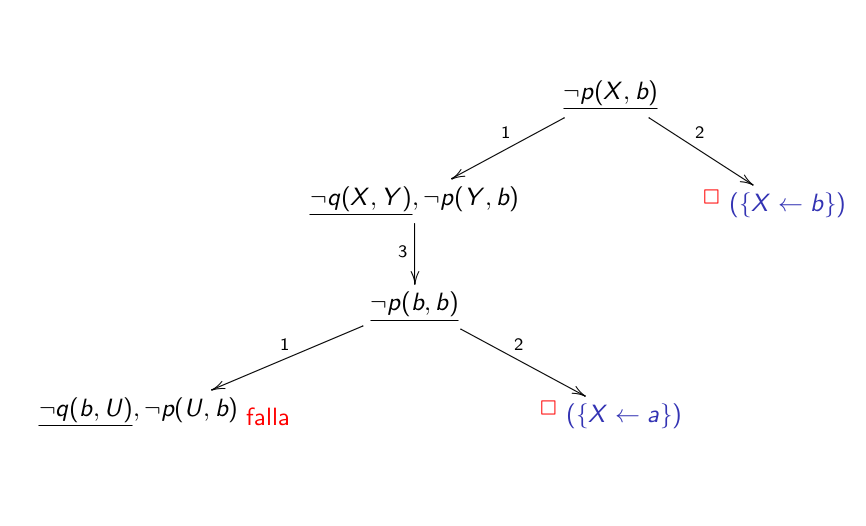
\includegraphics[scale=0.4]{imagenes/arbol_sld_prolog.png}

Otra posible estrategia de selección sería, por ejemplo, elegir resolver la cláusula más a la derecha, en cuyo caso el ejemplo que dimos dejaría de funcionar ya que la primer rama del árbol sería infinita y no encontrariamos nunca una refutación.

Y si decidiesemos seleccionar las cláusulas de abajo hacia arriba, entonces obtendriamos el árbol mostrado reflejado.

Hay que tener en cuenta que elegimos el ejemplo para que funcionase bien con la estrategia que sigue Prolog, sin embargo, hay ejemplos en lo que esta estrategia cae en el mismo caso que en la primer estrategia alternativa mencionada.

\subsubsection{Implementación y otras cosas sobre Prolog}
La estrategia usada por Prolog recorre el árbol SLD en \textbf{profundidad} (depth-first search). Las ventajas de esto es que puede ser implmentado de manera muy eficiente usando una \textbf{pila} para representar los átomos del goal.
La idea es hacer un \textbf{push} del resolvente del átomo del tope de la pila con la cláusula de definición y hacer un \textbf{pop} cuando el átomo del top de la pila no unifica con ninguna cláusula de definición más.

\subsubsection*{Cut}
Es una notación que nos permite \textbf{podar} el árbol SLD. Es de carácter extra-lógico y nos permite \textbf{hacer más eficientes} algunas consultas. El uso correcto de esta notación no debería modificar el universo de posibles soluciones a una consulta.

Cuando se selecciona un cut, tiene éxito \textbf{inmediatamente}. Si, debido a backtracking, se vuelve al mismo cut entonces se hace fallar el goal que le dio origen.

\subsection*{Negación por falla}
Se dice que un árbol SLD \textbf{falla finitamente} si es finito y no tiene ramas de éxito.

Dado un programa P el \textbf{conjunto de falla finita} de $P$ es $$\{ B ~|~B~ \text{ es un átomo cerrado y existe un árbol SLD que falla finitamente con } B \text{ como raíz}\} $$ 

Esto significa que podemos inferir la insatisfactibilidad de una cláusula cerrada si la cantidad de chequeos que tenemos que hacer para probarlo es finita y si, además, tenemos un conjunto finito de símbolos sobre los que chequear.

En Prolog, tenemos el predicado \textbf{not} que nos permite realizar este tipo de resolución, sin embargo debemos asegurarnos de que los predicados que le pasemos sean cerrados, ya que al no ser un predicado lógico, no se instancias variables en ningún momento.
\appendix
\newpage
\part{Apéndices}

\section{Programación funcional en Haskell}
\paragraph{Tipos elementales}
\begin{centrado}
	\begin{minted}{haskell}
1               -- Int          Enteros
'a'             -- Char         Caracteres
1.2             -- Float        Números de punto flotante
True            -- Bool         Booleanos
[1,2,3]         -- [Int]        Listas
(1, True)       -- (Int, Bool)  Tuplas, pares
length          -- [a] -> Int   Funciones
length [1,2,3]  -- Int          Expresiones
\x -> x         -- a -> a       Funciones anónimas
	\end{minted}
\end{centrado}

\paragraph{Guardas}
\begin{centrado}
	\begin{minted}{haskell}
signo n | n >= 0    = True
		| otherwise = False
	\end{minted}
\end{centrado}

\paragraph{Pattern Matching}
\begin{centrado}
	\begin{minted}{haskell}
longitud [] = 0
longitud (x:xs) = 1 + (longitud xs)
	\end{minted}
\end{centrado}

\paragraph{Polimorfismo paramétrico}
\begin{centrado}
	\begin{minted}{haskell}
todosIguales :: Eq a => [a] -> Bool
todosIguales [] = True
todosIguales [x] = True
todosIguales (x:y:xs) = x == y && todosIguales(y:xs)
	\end{minted}
\end{centrado}

\paragraph{Clases de tipo}
\begin{centrado}
	\begin{minted}{haskell}
Eq a    -- Tipos con comparación de igualdad
Num a   -- Tipos que se comportan como los números
Ord a   -- Tipos orden
Show a  -- Tipos que pueden ser representados como strings
	\end{minted}
\end{centrado}

\paragraph{Definición de listas}
\begin{centrado}
	\begin{minted}[breaklines]{haskell}
[1,2,3,4,5]                 -- Por extensión
[1 .. 4]                    -- Secuencias aritméticas
[ x | x <- [1..], esPar x ] -- Por compresión
		
cuando las usamos. Ejemplo de lista infinita:
		
infinitosUnos :: [Int]
infinitosUnos = 1 : infinitosUnos
		
puntosDelCuadrante :: [(Int, Int)]
puntosDelCuadrante = [ (x, s-x) | s <- [0..], x <-[0..s] ]
	\end{minted}
\end{centrado}

\paragraph{Funciones de alto orden}
\begin{centrado}
	\begin{minted}[breaklines]{haskell}
mejorSegun :: (a -> a -> Bool) -> [a] -> a
mejorSegun _ [x] = x
mejorSegun f (x : xs) | f x (mejorSegun f xs) = x
		| otherwise = mejorSegun f xs
	\end{minted}
\end{centrado}

\subsection{Otros tipos útiles}
\paragraph{Formula}
\begin{centrado}
	\begin{minted}[breaklines]{haskell}
data Formula = Proposicion String | No Formula 
		| Y Formula Formula
		| O Formula Formula
		| Imp Formula Formula
		
foldFormula :: (String -> a) -> (Formula -> a) -> 
(Formula -> Formula -> a) -> (Formula -> Formula -> a) 
-> (Formula -> Formula -> a) -> Formula -> a
foldFormula fp fn fy fo fImp form = case form of :
		Proposicion s -> fp s
		No sf -> fn (rec sf)
		Y sf1 sf2 -> fy (rec sf1) (rec sf2)
		O sf1 sf2 -> fo (rec sf1) (rec sf2)
		Impl sf1 sf2 -> fImpl (rec sf1) (rec sf2)
		where rec = foldForm fp fn fy fo fImp
	\end{minted}
\end{centrado}

\paragraph{Rosetree}
\begin{centrado}
	\begin{minted}[breaklines]{haskell}
data Rosetree = Rose a [Rosetree]
-- Hay varias formas de definir el fold para esta estructura
foldRose :: (a -> [b] -> b) -> Rosetree a -> b
foldRose f ( Rose x l ) = f x ( map ( foldRose f ) l )
		
foldRose2 :: ( a -> c -> b) -> ( b -> c -> c ) -> c 
-> Rosetree a -> b
foldRose2 g f z (Rose x l) = 
g x ( foldr f z ( map ( foldRose g f z ) l ) )
		
	\end{minted}
\end{centrado}


\newpage
\section{Extensiones del lenguaje \texorpdfstring{$\lambda^b$}{lambda b}}



\subsection{Registros \texorpdfstring{$\lambda^{...r}$}{lambda ...r}}

\paragraph{Tipos}
$$\sigma, \tau ~::=~...~|~\{l_i : \sigma_i ~^{i\in 1..n}\}$$

El tipo $\{l_i : \sigma_i^{i\in 1..n}\}$ representan las estructuras con $n$ atributos tipados, por ejemplo: $\{nombre : String,edad:Nat\}$
\paragraph{Términos}
$$ M~::=~ \dots~|~\{l_i = M_i ~^{i\in 1..n}\}~|~M.l $$

Los términos significan:
\begin{itemize}
	\item El registro $\{l_i = M_i ~^{i\in 1..n}\}$ evalua $\{l_i = V_i ~^{i\in 1..n}\}$  donde $V_i$ es el s al que evalúa $M_i$ para $i\in 1..n$.
	\item $M.l$: Proyecta el valor de la etiqueta $l$ del registro $M$
\end{itemize}

\paragraph{Axiomas y reglas de tipado}
\begin{equation*}
	\frac{\judgeType{\Gamma}{M_i}{\sigma_i} \text{ para cada } i \in 1..n}{\judgeType{\Gamma}{\{l_i = M_i ~^{i\in 1..n}\}}{\{l_i : \sigma_i ~^{i\in 1..n}\}}}(\text{T-RCD})
\end{equation*}
\vspace*{5mm}
\begin{equation*}
	\frac{\judgeType{\Gamma}{\{l_i = M_i ~^{i\in 1..n}\}}{\{l_i : \sigma_i ~^{i\in 1..n}\}}\hspace*{5mm} j \in 1..n}
	{\judgeType{\Gamma}{M.l_j}{\sigma_j}}(\text{T-Proj})
\end{equation*}

\paragraph{Axiomas y reglas de subtipado}
%\begin{equation*}
%	\frac{}{\{l_i : \sigma_i~|~i\in 1..n+k\} <: \{l_i : \sigma_i~|~i\in 1..n\}}(\text{S-RcdWidth})
%\end{equation*}
%
%\vspace*{5mm}
%\begin{equation*}
%	\frac{\sigma_i <: \tau_i\hspace*{5mm} i\in I = \{1..n\}}{\{l_i : \sigma_i\}_{i\in I} <: \{l_i : \tau_i\}_{i\in I}}(\text{S-RcdDepth})
%\end{equation*}

\begin{equation*}
	\frac{\{l_i| i\in 1..n\}\subseteq\{k_j|j\in 1..m\} \hspace*{5mm} k_j = l_i\Rightarrow \sigma_j <: \tau_i}{\{k_j:\sigma_j|j\in 1..m\} <: \{l_i:\sigma_i| i\in 1..n\}}(\text{S-Rcd})
\end{equation*}

\vspace*{5mm}
Esta regla nos dice que un registro $N$ es subtipo de otro registro $M$, si el conjunto de etiquetas de $M$ está contenido en el conjunto de etiquetas de $N$ y, además, si los tipos de cada una de esas etiquetas, en $M$, es más general que en $N$.

Una de las consecuancias de esta regla es que  $\sigma <\{\}$ para todo tipo registro $\sigma$. Esto es porque $\{\}$ no tiene etiquetas, osea que su conjunto de etiquetas es el conjunto $\emptyset$ que está contenido en todos los conjuntos.
\paragraph{Valores}
$$V~::=~\dots~|~\{l_i = V_i ~^{i\in 1..n}\}$$


\paragraph{Axiomas y reglas de evaluación}

\begin{equation*}
	\frac{j\in 1..n}{\{l_i = \lambdaValue{V_i} ~^{i\in 1..n}\}.l_j \to \lambdaValue{V_j}}(\text{E-ProjRcd})
\end{equation*}
\vspace*{5mm}
\begin{equation*}
	\frac{M \to M'}{M.l \to M'.l}(\text{E-Proj})
\end{equation*}

\vspace*{5mm}
\begin{equation*}
	\frac{M_j\to M_j'}{\{l_i = \lambdaValue{V_i}~^{i\in 1..j-1}, l_j = M_j, l_i = M_i ~^{i\in j+1..n}\} \to \{l_i = \lambdaValue{V_i}~^{i\in 1..j-1}, l_j = M'_j, l_i = M_i ~^{i\in j+1..n}\}}(\text{E-RCD})
\end{equation*}
\vspace*{5mm}
\subsection{Declaraciones Locales (\texorpdfstring{$\lambda^{...let}$}{lambda ...let})}\label{extension_lambda:let}

Con esta extensión, agregamos al lenguaje el término $\lambdaLet{x}{\sigma}{M}{N}$, que evalúa $M$ a un valor, liga $x$ a $V$ y, luego, evalúa $N$. Este término solo mejora la legibilidad de los programas que ya podemos definir con el lenguaje hasta ahora definido.

\paragraph{Términos}
$$ M~::=~ \dots~|~\lambdaLet{x}{\sigma}{M}{N} $$


\paragraph{Axiomas y reglas de tipado}
\begin{equation*}
	\frac{\judgeType{\Gamma}{M}{\sigma_1}\hspace*{5mm}\judgeType{\Gamma,x:\sigma_1}{N}{\sigma_2}}{\judgeType{\Gamma}{\lambdaLet{x}{\sigma_1}{M}{N}}{\sigma_2}}(\text{T-Let})
\end{equation*}

\paragraph{Axiomas y reglas de evaluación}

\begin{equation*}
	\frac{M_1\to M_1'}{\lambdaLet{x}{\sigma}{M_1}{M_2}\to \lambdaLet{x}{\sigma}{M'_1}{M_2}}(\text{E-Let})
\end{equation*}
\vspace*{5mm}
\begin{equation*}
	\frac{}{\lambdaLet{x}{\sigma}{\lambdaValue{V_1}}{M_2}\to \replaceBy{M_2}{x}{\lambdaValue{V_1}}}(\text{E-LetV})
\end{equation*}

\subsubsection{Construcción \textit{let} recursivo (Letrec)}
Una construcción alternativa para definir funciones recursivas es 
$$letrec~f:\sigma\to\sigma = \lambdaAbs{x}{\sigma}{M~in~N}$$

Y $letRec$ se puede definir  en base a $let$ y $fix$ (definido en \ref{lambda_calculo:recursion}) de la siguiente forma:

$$\lambdaLet{f}{\sigma\to\sigma}{(\lambdaFix{\lambdaAbs{f}{\sigma\to\sigma}{\lambdaAbs{x}{\sigma}{M}}})}{N}$$

\subsection{Tuplas}

\paragraph{Tipos}
$$\sigma,\tau~::= \dots~|~\sigma\times\tau$$

\paragraph{Términos}
$$M,~N~::=~\dots~|~<M,N>~|~\pi_1(M)~|~\pi_2(M)$$
\paragraph{Axiomas y reglas de tipado}
\begin{equation*}
	\frac{\judgeType{\Gamma}{M}{\sigma}\hspace*{5mm}\judgeType{\Gamma}{N}{\tau}}{\judgeType{\Gamma}{<M,N>}{\sigma\times\tau}}(\text{T-Tupla})
\end{equation*}
\vspace*{5mm}
\begin{equation*}
	\frac{\judgeType{\Gamma}{M}{\sigma\times\tau}}{\judgeType{\Gamma}{\pi_1(M)}{\sigma}}(\text{T-}\pi_1)\hspace*{1cm}\frac{\judgeType{\Gamma}{M}{\sigma\times\tau}}{\judgeType{\Gamma}{\pi_2(M)}{\tau}}(\text{T-}\pi_2)
\end{equation*}

\paragraph{Valores}
$$V~::=~\dots~|~<V,V>$$

\paragraph{Axiomas y reglas de evaluación}
\begin{equation*}
	\frac{M\to M'}{<M,N>\to<M',N>}(\text{E-Tuplas})\hspace*{1cm}\frac{N\to N'}{<\lambdaValue{V},N>\to<\lambdaValue{V},N'>}(\text{E-Tuplas1})
\end{equation*}
\vspace*{5mm}
\begin{equation*}
	\frac{M\to M'}{\pi_1(M)\to\pi_1(M')}(\text{E-}\pi_1)\hspace*{1cm}\frac{}{\pi_1(<\lambdaValue{V_1}, \lambdaValue{V_2}>)\to\lambdaValue{V_1}}(\text{E-}\pi'_1)
\end{equation*}
\vspace*{5mm}
\begin{equation*}
	\frac{M\to M'}{\pi_2(M)\to\pi_2(M')}(\text{E-}\pi_2)\hspace*{1cm}\frac{}{\pi_2(<\lambdaValue{V_1}, \lambdaValue{V_2}>)\to\lambdaValue{V_2}}(\text{E-}\pi'_2)
\end{equation*}

\subsection{Árboles binarios}

\paragraph{Tipos}
$$\sigma,\tau~::= \dots~|~AB_\sigma$$

\paragraph{Términos}
$$M,~N~::=~\dots~|~\text{Nil}_\sigma~|~\text{Bin}(M, N, O)~|~\text{raiz}(M)~|~\text{der}(M)~|~\text{izq}(M)~|~\text{esNil}(M)$$
\paragraph{Axiomas y reglas de tipado}
\begin{equation*}
	\begin{gathered}
		\frac{}{\judgeType{\Gamma}{\text{Nil}_\sigma}{AB_\sigma}}(\text{T-Nil})\hspace*{1cm}
		\frac{\judgeType{\Gamma}{M}{AB_\sigma}\hspace*{5mm}\judgeType{\Gamma}{N}{\sigma}\hspace*{5mm}\judgeType{\Gamma}{O}{AB_\sigma}}{\judgeType{\Gamma}{\text{Bin}(M, N, O)}{AB_\sigma}}(\text{T-Bin}) \\
		\vspace*{5mm}\\
		\frac{\judgeType{\Gamma}{M}{AB_\sigma}}{\judgeType{\Gamma}{\text{raiz}(M)}{\sigma}}(\text{T-raiz})\hspace*{1cm}
		\frac{\judgeType{\Gamma}{M}{AB_\sigma}}{\judgeType{\Gamma}{\text{der}(M)}{AB_\sigma}}(\text{T-der})
		\vspace*{5mm} \\
		\frac{\judgeType{\Gamma}{M}{AB_\sigma}}{\judgeType{\Gamma}{\text{izq}(M)}{AB_\sigma}}(\text{T-izq})
		\hspace*{1cm}
		\frac{\judgeType{\Gamma}{M}{AB_\sigma}}{\judgeType{\Gamma}{\text{isNil}(M)}{Bool}}(\text{T-isNil})
	\end{gathered}
\end{equation*}

\paragraph{Valores}
$$V~::=~\dots~|~\text{Nil}~|~\text{Bin}(V,V,V)$$

\paragraph{Axiomas y reglas de evaluación}
\begin{equation*}
	\frac{M\to M'}{\text{Bin}(M,N,O)\to \text{Bin}(M',N,O)}(\text{E-Bin1})\hspace*{1cm}\frac{N\to N'}{\text{Bin}(V,N,O)\to \text{Bin}(V,N',O)}(\text{E-Bin2})
\end{equation*}
\vspace*{5mm}
\begin{equation*}
	\frac{O\to O'}{\text{Bin}(V_1,V_2,O)\to \text{Bin}(V_1,V_2,O')}(\text{E-Bin3})
\end{equation*}
\vspace*{5mm}
\begin{equation*}
	\frac{M\to M'}{\text{raiz}(M)\to\text{raiz}(M')}(\text{E-Raiz1})\hspace*{1cm}\frac{}{\text{raiz}(\text{Bin}(V_1,V_2,V_3))\to V_2}(\text{E-Bin3})
\end{equation*}
\vspace*{5mm}
\begin{equation*}
	\frac{M\to M'}{\text{der}(M)\to\text{der}(M')}(\text{E-Der1})\hspace*{1cm}\frac{}{\text{der}(\text{Bin}(V_1,V_2,V_3))\to V_3}(\text{E-Der2})
\end{equation*}
\vspace*{5mm}
\begin{equation*}
	\frac{M\to M'}{\text{izq}(M)\to\text{izq}(M')}(\text{E-Izq1})\hspace*{1cm}\frac{}{\text{izq}(\text{Bin}(V_1,V_2,V_3))\to V_1}(\text{E-Izq2})
\end{equation*}
\hspace*{5mm}
\begin{equation*}
	\frac{}{\text{isNil}(M)\to\text{izq}(M')}(\text{E-isNil1})\hspace*{1cm}\frac{}{\text{isNil}(\text{Bin}(V_1,V_2,V_3))\to false}(\text{E-isNilBin})
\end{equation*}
\hspace*{5mm}
\begin{equation*}
	\frac{}{\text{isNil}(\text{Bin}(V_1,V_2,V_3))\to true}(\text{E-isNilNil})
\end{equation*}

\newpage
\section{Javascript}
\paragraph{Declaración de variables}
\begin{centrado}
	\begin{minted}{javascript}
	// Declaración de variables
	let miVar = 1;
	var suVar = 2;
	
	// Declaración de constante, no pueden ser modificadas.
	const miConstante = 3; 
	\end{minted}
\end{centrado}

Y es \textbf{case-sensitive}, es decir \texttt{unavariable} y \texttt{unaVariable} no son las mismas variables.

\paragraph{Tipos primitivos}

\begin{itemize}
	\item \texttt{number}: Los números, no hay distinción entre enteros y punto flotantes. Contiene a las constantes \texttt{-Infinity},\texttt{+Infinity}, \texttt{NaN}.
	\item \texttt{boolean}: Los literales \texttt{true} y \texttt{false} con las operaciones \texttt{\&\&}, \texttt{!} y \texttt{||}.
	\item \texttt{string}: Secuencias de cero o más carácteres entre comillas simples o dobles.
	\item \texttt{null}: Un único valor \texttt{null} (nada, valor desconocido).
	\item \texttt{undefined}: Un único valor \texttt{undefined} (el valor no está definido).
\end{itemize}

\end{document}